\documentclass[12pt,a4paper,final,oneside,openany]{memoir}

\usepackage[lang=en,grid]{kufront}
\usepackage[english]{babel}
\usepackage[utf8]{inputenc}
\usepackage[T1]{fontenc}
\usepackage[british]{isodate}
\usepackage{booktabs}
\usepackage{fixltx2e}
\usepackage{nameref}
\usepackage{amsmath}
\usepackage{amssymb}
\usepackage{mathtools}
\usepackage[lofdepth,lotdepth]{subfig}
\usepackage{multirow}
\usepackage{float}
\usepackage{hyperref}
\usepackage{color}
\usepackage{cite}
\usepackage{url}
\usepackage[verbose]{wrapfig}
\usepackage[ruled,vlined]{algorithm2e}
\usepackage{multirow}
\usepackage{booktabs}
\usepackage{array}
\usepackage{footnote}
\usepackage{amsthm}
\usepackage{lettrine}
\usepackage[labelfont=bf]{caption}
\usepackage{listings}
\usepackage{afterpage}
\usepackage{lastpage}
\usepackage{mdframed}
\usepackage{booktabs}
\usepackage{xcolor}
\usepackage{ifthen}

\definecolor{generalcolor}{RGB}{52,73,94}
\definecolor{myblue}{HTML}{268BD2}
\definecolor{mygreen}{HTML}{859900}
\definecolor{mygray}{HTML}{93A1A1}

\definecolor{sourcebackground}{HTML}{ECF0F1}
\definecolor{bashcommetcolor}{HTML}{95A5A6}

\newtheorem{theorem}{Theorem}

\theoremstyle{definition}
\newtheorem{definition}{Definition}[section]

\def \CodeName{SOFA }
\def \CodeNameShort{SOFA}
\def \CodeNameFull{SOFA (Semantic Oriented File Archive) }

\def \FullName{Steffen Karlsson}
\def \HandinDate{August 2016}

\makeatletter
\newcommand\footnoteref[1]{\protected@xdef\@thefnmark{\ref{#1}}\@footnotemark}
\makeatother

\renewcommand{\kufrontfont}{\sffamily}

\renewcommand{\lstlistingname}{Code}

\title{\CodeName}
\subtitle{\large A semantic oriented file archive for big data analysis}
\author{\Large \FullName \quad {\ttfamily\large ckh340@alumni.ku.dk}}
\date{\HandinDate}
\project{\bfseries\LARGE Master's Thesis}
\supervisor{\textbf{Supervisor:} Professor Brian Vinter}

\renewcommand*{\cftpartname}{Part\space}
\cftpagenumbersoff{part}

\newcommand{\subimgwidth}{.5\textwidth}
\newcommand{\imgwidth}{.8\textwidth}

\def\thefigure{\arabic{figure}}
\setcounter{tocdepth}{1}

\renewcommand{\LettrineFontHook}{\sffamily}

\newcommand\textlc[1]{\MakeLowercase{#1}}
\newcommand\BigLetter[2]{\lettrine[lines=2, loversize=0.2, findent=0.2em]{\textbf{#1}}{}\textlc{#2}}

\newcommand{\todo}[1]{{\color{red} \textbf{TODO:}} #1}

\newcommand{\reference}[2]{outlined in Definition \ref{#1} and described in further details in Section \ref{#2}}

\newcommand{\etal}{\textit{et al}. }
\newcommand{\ie}{\textit{i}.\textit{e}., }
\newcommand{\eg}{\textit{e}.\textit{g}. }

\lstset{ %
  basicstyle=\footnotesize,        % the size of the fonts that are used for the code
  breaklines=true,                 % sets automatic line breaking
  captionpos=b,                    % sets the caption-position to bottom
  commentstyle=\color{mygreen},    % comment style
  escapeinside={\%*}{*)},          % if you want to add LaTeX within your code
  frame=none,                      % adds a frame around the code
  keywordstyle=\color{blue},       % keyword style
  language=Python,                 % the language of the code
  numbers=left,                    % where to put the line-numbers; possible values are (none, left, right)
  numbersep=5pt,                   % how far the line-numbers are from the code
  numberstyle=\tiny\color{mygray}, % the style that is used for the line-numbers
  rulecolor=\color{black},         % if not set, the frame-color may be changed on line-breaks within not-black text (e.g. comments (green here))
  stepnumber=2,                    % the step between two line-numbers. If it's 1, each line will be numbered
  showspaces=false,
  tabsize=2,                       % sets default tabsize to 2 spaces
  title=\lstname,                   % show the filename of files included with \lstinputlisting; also try caption instead of title
  xleftmargin=.02\textwidth
}

\newcommand{\cfigure}[4]{
	\vspace*{5mm}
	\begin{figure}[ht!]
		\centering
		\includegraphics[scale=#4]{pdf/#1}
		\caption[#3]{#2 \label{fig:#1}}
	\end{figure}
}

\newmdenv[
  topline=false,
  bottomline=false,
  skipabove=\topsep,
  skipbelow=\topsep,
  leftmargin=2pt,
  rightline=false,
  innertopmargin=6pt,
  innerbottommargin=10pt
]{siderules}

\newcommand{\testcase}[7]{
	\vspace*{4mm}
	\begin{siderules}
	{\large\sffamily\textbf{Test Case:}} #1
	\begin{quotation}
		\textit{#2}
	\end{quotation}
	\begin{quotation}
		\vspace*{2mm}
		\ifthenelse { \equal {#3} {} } {} {
			\noindent
			\textbf{Note}: #3
			\\~
			\\~
			\vspace*{2mm}}
		\noindent
		\textbf{Arguments}:
		#4
		\vspace*{2mm}
		\noindent
		\textbf{Expected result}:
		\begin{quotation}
			#5
		\end{quotation}
		\vspace*{2mm}
		\noindent
		\textbf{Result}\ifthenelse { \equal {#6} {} } {:} { (\textit{#6}):}
		\vspace*{2mm}
		\begin{quotation}
			#7
		\end{quotation}
	\end{quotation}
	\end{siderules}
}

\usepackage{tikz, blindtext}
\makechapterstyle{box}{
  \renewcommand*{\printchaptername}{}
  \renewcommand*{\chapnumfont}{\normalfont\sffamily\huge\bfseries}
  \renewcommand*{\printchapternum}{
    \flushright
    \begin{tikzpicture}
      \draw[fill,color=black] (0,0) rectangle (1.5cm,1.5cm);
      \draw[color=white] (0.75cm,0.75cm) node { \chapnumfont\thechapter };
    \end{tikzpicture}
  }
  \renewcommand*{\chaptitlefont}{\normalfont\sffamily\Huge\bfseries}
  \renewcommand*{\printchaptertitle}[1]{\flushright\chaptitlefont##1}
}

\renewcommand*{\chaptitlefont}{\normalfont\sffamily\Huge\bfseries}

\let\Sectionmark\sectionmark
\def\sectionmark#1{\def\Sectionname{#1}\Sectionmark{#1}}

\makepagestyle{diku}
\makeevenhead{diku}{\sffamily\rightmark}{}{}
\makeoddhead{diku}{\sffamily\rightmark}{}{\sffamily\Sectionname}
\makeevenfoot{diku}{}{\sffamily\thepage \text{ of } \sffamily\pageref{LastPage}}{}
\makeoddfoot{diku}{}{\sffamily\thepage \text{ of } \sffamily\pageref{LastPage}}{}
\makeheadrule{diku}{\textwidth}{1pt}
\makeheadposition{diku}{flushright}{flushright}{}{}   

\begin{document}
\pagestyle{empty}
\frontmatter
\clearpage

\maketitle
\clearpage

\pagestyle{plain}
\vspace{3cm}
\addcontentsline{toc}{chapter}{Abstract}
\begin{abstract}
The goal of the project is to design and implemented a file archive for big data analysis with high performance and scientific data in mind. Existing MapReduce\cite{Dean:2008:MSD:1327452.1327492} frameworks such as the commonly used Apache Hadoop\cite{PageHadoop} is designed and developed for different purposes than what they are used for nowadays. 

The conventional file system approach with fixed size data blocks implemented in Hadoop makes it suboptimal for scientific data processing because splitting data at arbitrary positions means that high-level data structures such as NetCDF data and multidimensional arrays are distributed across multiple machines. A consequence of this is increased latency and intercommunication between machines during data processing.
\newline

Hadoop has previously been investigated and evaluated speci\-fically for scientific data-intensive operations\cite{fadika2012evaluating} and even extended and modified for individual use-case such as NetCDF\cite{buck2011scihadoop}.
\newline

This project introduces \CodeNameShort, a distributed semantic oriented file archive for big data analysis that preserves the structure of data by jointly storing semantically coherent data parts of arbitrary size. The responsibility of correctly splitting the data is transitioned towards the end-user and thus not inaccurately made by the system. The system will be targeted inexpensive commodity hardware like other similar frameworks and will thus primarily rely on the underlying file system for redundancy and hardware for recovery.
\newline

The \CodeName framework provides a range of different system customizations and data related opportunities such as instance based virtualization and the unique and innovative opportunity of virtual replication at a data level specified independently for each entry, 	instead of at a machine level. The framework provides a public available core API that exposes a vast amount of high level routines for developing powerful and useful extensions and applications. The project introduces such an extension BDAE (\textit{/b'dei'/}) which models the notion of a data access and processing layer for \CodeNameShort.

\end{abstract}

\setlength{\cftpartnumwidth}{4em}

\chapter{Preface}
\chapter{Preface}

\clearpage
\tableofcontents*

\clearpage
\listoffigures*

\mainmatter
\chapterstyle{box}
\pagestyle{diku}

\counterwithout{table}{chapter}
\counterwithout{figure}{chapter}

\chapter{Introduction}
\BigLetter{A}{ progressively} increasing challenge in high performance computing (HPC) is how to store the large amount of data on disk efficiently, especially with the ubiquitous enthusiasm for Big Data Analysis (BDA) frameworks, within the area of influence. A commonly used distributed computation framework for BDA is Apache's Hadoop\cite{PageHadoop}, where data access is based on the Hadoop Distributed File System (HDFS) \cite{Shvachko:2010:HDF:1913798.1914427} and the primary execution model is based on MapReduce\cite{Dean:2008:MSD:1327452.1327492}. These frameworks are developed under different circumstances, and with different purposes compared to what they are presently used.
\newline

HDFS, as well as the Google File System \cite{Ghemawat:2003:GFS:945445.945450}, follows a centralized architectural master/slave organization (described in \cite{Tanenbaum:2006:DSP:1202502} and briefly in \cite{Wilkinson:1998:PPT:289352}) where what is denoted as NameNode acts as the master. This server maintains attributes such as permissions and namespace tree for slaves. Also, it implements a proxy to handle operations realised on the file system at the slaves. 
\newline

Writing to the Hadoop file system can likely cause what's known as the data residual problem (Figure \ref{fig:data-residual}). Thus, semantically correlated or coherent data can be distributed across different servers. Hadoop is implemented using a conventional file system approach, \ie fixed sized blocks of 64MB. 
\newpage

\begin{figure}
	\centering
	\hspace*{15mm}
	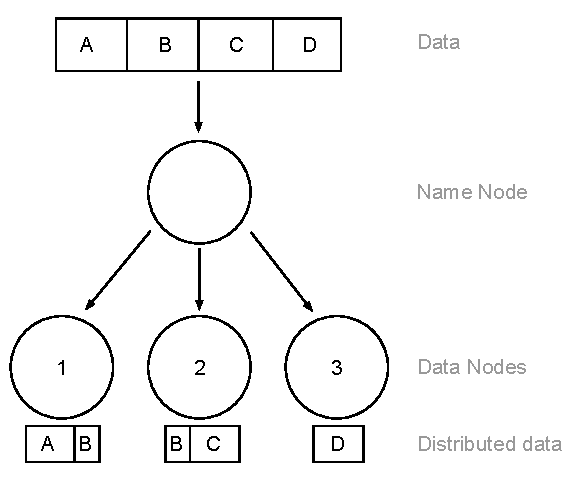
\includegraphics[scale=0.8]{pdf/data-residual.pdf}
	\caption[HDFS data residual problem]{HDFS data residual problem which ultimately requires Data Node 1 and 2 to exchange data for a consistent processing of block B, leading to an increased I/O cost. \label{fig:data-residual}}
\end{figure}

As a matter of fact, the only case where data partitioning is ensured to be avoided is when the \textit{size of the data} modulo \textit{the block size} is equal to zero. As a consequence, individual computer scientist are required to implement a network communication protocol between the slaves to handle this problem, which typically causes increased latency. The goal is to ensure a consistent view and process of the coherent data representations.

\section{Problem definition} \label{sec:problem}
\begin{quotation}
\hspace*{-7mm}
\textit{Firstly, analyze and investigate whether a distributed parallel file system that efficiently hides latency and reduce IO-cost is feasible. Secondly, if such a system is feasible implement a prototype in a sensibly selected language, architecture and environment.} \newline
\end{quotation}

\section{Related work} \label{sec:related}
Existing implementations and research projects within the field of big data analysis frameworks and distributed parallel file systems relevant to this project will be described in this section, including the once previously mentioned.

\subsection*{Hadoop}
Hadoop was originally described in 2010 by Shvachko \etal \cite{Shvachko:2010:HDF:1913798.1914427}. The Apache and Yahoo! developed framework is designed to store and analyze enormous datasets. It provides the distributed hierarchical file system with directories and archives HDFS, as data access layer (DAL) and a primary execution model based on the programming paradigm MapReduce (sharing this feature with the following computing platform), outlined in Definition \ref{def:mapreduce}.
\vspace*{2mm}

\begin{definition}[MapReduce] \label{def:mapreduce}
\textit{A programming paradigm and an associated implementation presented by Dean and Ghemawat} \cite{Dean:2008:MSD:1327452.1327492} \textit{used for data generation, analysis and processing. Fundamentally it is assembled by two separate user specified functions:} \texttt{map} \textit{and} \texttt{reduce}\textit{, which at execution time are parallelized automatically.}
\end{definition}
\vspace*{2mm}

HDFS implements a master/slave architecture where the NameNode server acts as the master and the DataNodes are the slaves. Metadata and application data are stored separately on respectively master and slave. Having a stateful master without replication is a single point of failure  as described by Yahoo! in the Hadoop developer tutorial:

\begin{quotation}
	\textit{"The single point of failure in a Hadoop cluster is the NameNode $\ldots$ loss results in cluster unavailability. The permanent loss of NameNode data would render the cluster's HDFS inoperable."}\cite{YahooDocumentation}
\end{quotation}

Additionally it's a potential bottleneck in a system, but in this project it's a tradeoff between throughput and accessibility.

\subsection*{Facebook (Hadoop)}
Approximately 40\% percentage of all incidents at the Facebook Data Warehouse is somewhat Hadoop related (Figure \ref{fig:fb-hadoop-incidents}), many of those is due to the single point of failure (SPOF) error at the NameNode, which causes more or less the whole Hadoop cluster to be unavailable and thus not correctly functioning. Improving HDFS and SPOF error at the NameNode is therefor an essential task to ensure that the ecosystem are efficient and reliable.

\begin{figure}[h!]
	\centering
	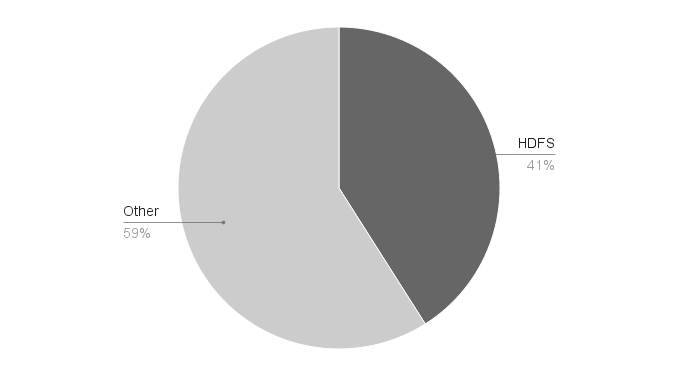
\includegraphics[scale=0.48]{img/fb-hadoop-incidents.png}
	\caption[Incidents at Facebooks Data Warehouse]{Incidents at Facebooks Data Warehouse by percentage at the responsible part, others including user specified jobs etc.\cite{FacebookHadoopImprovement}. \label{fig:fb-hadoop-incidents}}
\end{figure}

\newpage
Facebooks engineers designed a solution based on a so-called Avatar\-node, as a functioning hot fail-over solution, turning the existing NameNode into a highly-available server. The open source Avatarnode is essentially two NameNodes wrapped in an Apache ZooKeeper\footnote{Apache ZooKeeper\cite{PageZookeper} is a centralized service provider for configuration information and naming etc.} instance, with support for manual failover. The two NameNode instances behave as an active one and a standby with internal virtual IP address (VIP), handled by ZooKeeper, \ie each client request is initialized through that to get the VIP of the primary node (Figure \ref{fig:facebook-avatarnode}).
\newline

Synchronization between the active and the standby NameNode instance is managed by a NFS (Network File Server).
\vspace*{3mm}

\begin{figure}[h!]
	\centering
	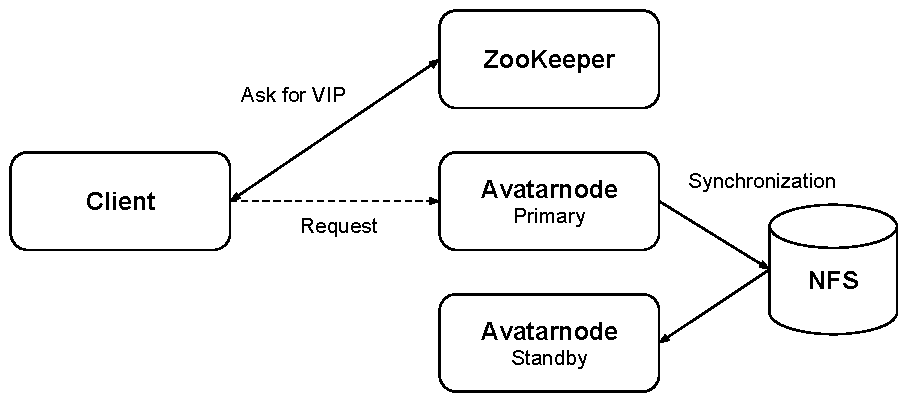
\includegraphics[scale=0.8]{pdf/facebook-avatarnode.pdf}
	\caption[Avatarnode: Facebooks Hadoop implementation]{Control flow of the AvatarNode and ZooKeeper with virtual IP address and network file server for synchronization. \label{fig:facebook-avatarnode}}
	\vspace*{3mm}
\end{figure}

Facebook claims that the solution leads to a projected result of 50\% lesser planned downtime, \ie a critical time where that part of the warehouse is unavailable. Though, one could certainly come up with new issues arising in this solution:
\begin{itemize}
	\item SPOF error reliability of the Apache ZooKeeper instance, since that is the only access-point now.
	\item SPOF error reliability of the NFS.
\end{itemize}

\subsection*{Hadoop 2.x}
Apache later released in Hadoop \textbf{2.x} \cite{Hadoop2xDocumentation} their solution to the single point of failure problem which they have described as: 

\begin{quotation}
	\textit{"$\ldots$ if that machine or process became unavailable, the cluster as a whole would be unavailable until the NameNode was either restarted or brought up on a separate machine"}. 
\end{quotation}

The solution is based on redundant duplication of the NameNode, such that one machine acts as the active one serving clients and another as the full redundant standby, which allows a fast fail-over in the case that the Active one crashes. The synchronization of logs and state between the two masters can be accomplished in two different ways:
\vspace*{3mm}

\begin{enumerate}
	\item Having at least 3 or more relatively lightweight Quorum Journal Manager (QJM) daemons to tolerate the failure of a single machine, because each modification has to be written to a quorum based majority of the daemons
	
	Major problems in this solution are:
\begin{itemize}
	\item Synchronization (the communication or latency cost of it).
	\item Considerable increase in hardware\footnote{One new machine for the standby and presumably three for the QJMs.}.
\end{itemize}
	\vspace*{3mm}
	
	\item Another option is to use a shared network file server (NFS) storage (Figure \ref{fig:hadoop-2x-nfs}).
	\begin{figure}[h!]
		\centering
		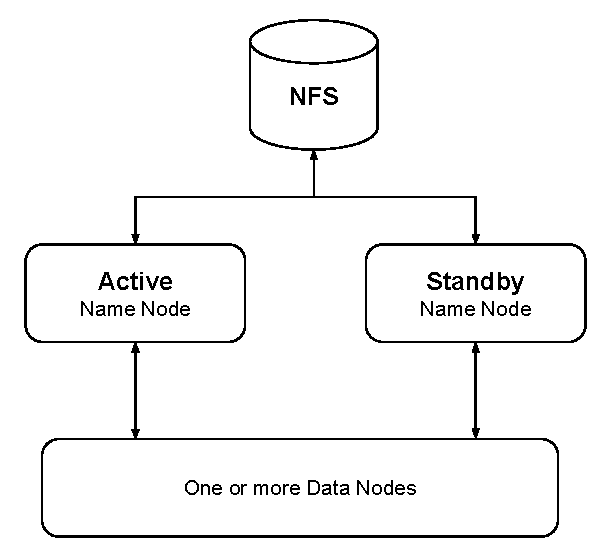
\includegraphics[scale=0.6]{pdf/hadoop-2x-nfs.pdf}
		\caption[Hadoop 2.x NFS solution]{Component diagram of the Hadoop 2.x NFS solution. \label{fig:hadoop-2x-nfs}}
	\end{figure}	

	This approach will undeniably mask the single point of failure (SPOF) error on the NameNode master by the cost and reliability to handle SPOF errors on the network file system abstraction, which in fact in most cases is a single server.
\end{enumerate}

\subsection*{Disco}
Mundkur \etal at Nokia Research Center published in 2011 a paper on their implementation of the distributed computing platform Disco\cite{PageDisco}\cite{Mundkur:2011:DCP:2034654.2034670}. Disco is an easy customizable MapReduce (Defintion \ref{def:mapreduce}) framework with regards to environment and requirements, designed for clusters of commodity server machines. Disco is likewise based on the master/slave architecture and relies on a standard file system and thus, deprioritizes persistent fault tolerance, achievable by a dedicated custom implementation. 
\newline

The single master pattern is as mentioned a single point of failure but is preferred due to consistency over availability (CAP theorem is outlined in \ref{def:cap}).
\vspace*{2mm}

\begin{definition}[CAP Theorem] \label{def:cap}
\textit{Eric Brewer presented in his keynote speech}\cite{Brewer2000} \textit{the CAP (Consistency, Availability, and Partition Tolerance) theorem that states, a distributed system (set of independent computers working together) only at any point in time can guarantee two of the three listed acronym properties, as illustrated in Figure \ref{fig:cap}.}

\begin{figure}[h!]
	\centering
	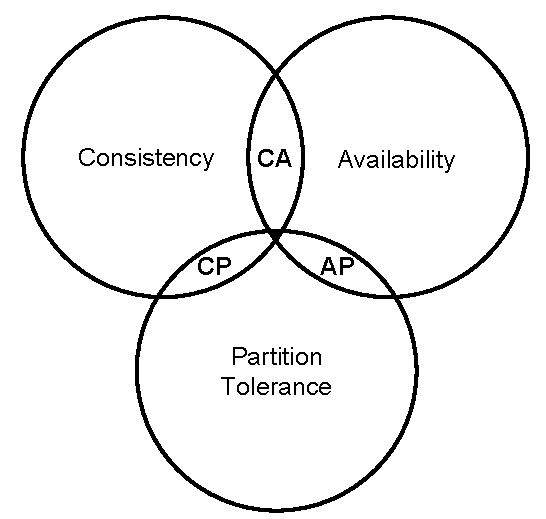
\includegraphics[scale=0.7]{pdf/cap.pdf}
	\caption{Illustrating the concept and limitations of CAP. \label{fig:cap}}
\end{figure}	
\end{definition}

\subsection*{Dynamo}
Dynamo is a highly available key-value storage system presented by Amazon engineers \cite{DeCandia:2007:DAH:1294261.1294281}. The system is implemented using an eventual consistency protocol and thereby sacrifices it under certain scenarios, by cause of availability. 

The reason for this choice is the \textit{"always-on"} user experience on core services on the Amazon platform that Dynamo is used to function. Dynamo uses consistent hashing (Definition \ref{def:ch}) to partition the key space across all available machines. A uniform distribution ultimately leads to a uniform load, assuming the key space access is not too skewed.
\vspace*{3mm}

\begin{definition}[Consitent hashing] \label{def:ch}
\textit{Engineer at Apache, White, describes in his blog post} \cite{PageWhiteCH} \textit{the purpose and demand for consistent hashing. It arose from the problems and limitations experienced with a naive hash-based key space distribution in a distributed system, where adding and removing machines in the network can be a catastrophe from a network bandwidth point of view, due to redistribution of the key space. In consistent hashing, only a fair share proportion from each of the machines is reassigned, while adding or removing machines.}
\end{definition}

\subsection*{Google File System}
Ghemawat \etal at Google describes the scalable distributed file system (GFS: Google File System) designed at implemented for primary developed for internal usage \cite{Ghemawat:2003:GFS:945445.945450}. 

The file system is designed to run on inexpensive commodity hardware like Dynamo and to provide fault tolerance. The architecture is a single stateful master and slave(s) organization, where the (GFS) master maintains all metadata file in the system. 
\newline

A vastly simplified design and sophisticated placement of data on the slaves, together with a strong recovery protocol has been prioritized compared to the risk of a single master (as previously explained). Communication between clients and the master are also widely reduced, by caching slave metadata for further intercommunication on the client eliminating the bottleneck effect on the master.
\vspace*{3mm}

\begin{definition}[Bottleneck effect] \label{def:bottle}
\textit{A part of a system is defined as a bottleneck if it critically limits the remaining system. This component usually has the lowest throughput of all.}
\end{definition}

\section{Proposal} \label{sec:proposal}
The knowledge, features, and compromises in the papers discussed and described in Related work provides the foundation for the research in the project. The ambition of the research is to first of all design a prototype of an alternative to the existing file archives used in big data analysis and secondly if possible to implement it.
\newline

The design of the architectural organization of the prototype is intended to eliminate the complications and issues in the existing solutions that has been described. A desired outcome is a substitute system eliminating data residuals with reduced I/O-cost and complexity and increased performance.
\newline

This can be achieved by splitting data semantically coherent at key positions by the file system, thus, data will be divided into arbitrarily sized chunks instead of fixed. Main challenges includes:
\vspace*{2mm}
\begin{itemize}
	\item Describing a domain specific model to characterize the data semantics.
	\item Defining a direct data mapping for storing and retrieval.
	\item Designing a system that scales as the data and request rate grows, \ie provides consistent and intelligent load balancing.
\end{itemize}

A feasible solution to reduce I/O-cost includes the mechanism of data cleaning, which is an important preprocessing step in big data analysis where \ie following actions can be performed:
\begin{itemize}
	\item Reformatting multidimensional scientific dataset such that identical features are grouped.
	\item Reducing noise.
	\item Transformation and dimensionality reduction (remove redundancy).
\end{itemize}
\vspace*{5mm}

The system seeks to perform the actions as mentioned above in real time since they are computationally simple on modern high-end processors and are attractive to perform before writing data to disk. 
\newline

Furthermore, a straightforward extension is to measure and store elemental statistics per dataset in a fashionable and state-of-the-art way. It is ultimately an ambition to integrate the same execution model as in \eg Hadoop and Disco, namely MapReduce around the implemented file archive to compose a full big data analysis framework alternative.

\section{Assumptions} \label{sec:assumption}
Following assumptions are constructed first and foremost to limit the prototype to the field of study relevant for this project and secondly to match the surrounding environment and settings.

\begin{itemize}
	\item The solution is targeted research and scientific datasets. 
	\item The solution is targeted and used for big data analysis.
	\item A full dataset is accessed, processed or modified at once.
	\item Individual data entries can be processed and analyzed independently and the order of data entries is irrelevant.
	\item The majority of the datasets are passive, \eg not quite accessed as much as expected in systems like GFS.
\end{itemize}

\section{Outline}
Part \ref{prt:sofa} explains the needs and requirements of the file archive for big data analysis based on the knowledge learned from analysis existing solutions in Chapter \ref{sec:introduction}. Additionally, it describes the architecture and design along with the implementation of the prototype. Part \ref{prt:extensions} explains the implementation of an extension build on top of the file archive based on the API described in Chapter \ref{chp:api}. Part \ref{prt:evaluation} finally, validates the correctness and measures the efficiency of the final solutions in addition to describing the plans for the future.

\part{A Semantic Oriented File Archive} \label{prt:sofa}
\chapter{Analysis} \label{chp:analysis}
\BigLetter{I}{nteresting} aspects of system design, architecture, and infrastructure from existing big data analysis computational frameworks will be examined in this chapter. Prior architecture presumptions and objectives will additionally be formulated to restrict the scope of the prototype but also to indicate the area of importance. 

Generalized test data within the addressed research areas will subsequently be presented. Those will collectively contribute to a comprehensive investigation challenging various aspects of the project.
\newline

Big data analysis (BDA) is widely used in most research areas, and businesses and the volume, variety, and velocity that data are progressing will continue expanding. The demand for processing large amount data has never been bigger; this includes cracking hidden patterns, unknown correlations and seeking new valuable information.

\section{Observations}
Hadoop (Section \ref{sec:related}), one of the most widely used large-scale frameworks for BDA is characterized in \cite{Mundkur:2011:DCP:2034654.2034670} as \textit{"rather heavyweight and difficult to adapt to custom environments"}. 

Supercomputing enthusiast Glenn Lockwood describes in his blog post \cite{PageLockwoodHadoop} that high-performance computing (HPC) communities keep having troubles understanding the match between Hadoop and HPC. The reason is that it isn't designed with HPC in mind and is developed under other circumstances, and for another purpose than what it is used for nowadays. Additionally, it is written in the programming language Java which core feature is the fact that it is platform-independent \cite{PageJava}, a concept that is completely opposite to HPC where it is favored to optimize code for specific hardware.

\section{Single Master}
A vast majority of the computing platforms discussed in Section \ref{sec:related} are based on a master/slave architecture where the specific master is stateful and could be a potential bottleneck (Definition \ref{def:bottle}) in the system. Additionally is such setting also a single point of failure (SPOF) error, meaning that a fail or crash can be fatal, expensive, or even a catastrophe.
\newline

The single master pattern in Hadoop at the earlier versions (before \textbf{2.x}) was a serious issue because the stateful master that keeps the entire namespace in random access memory (RAM) did not support automatic fail-over. Although the master periodically persists namespace state on disk as a system-record image and moreover keeps a synchronized log of all events too, it is required replay the record and the logs at a restart to recover the global state.

Later versions support fail-over to a working redundant standby copy, with hardware and communication cost. Other solutions to the SPOF error (Section \ref{sec:related}) such as the Facebook Avatarnode Hadoop extension requires integrations and instances of extra systems like ZooKeeper.
\newline

Systems like the Google File System follows the same stateful metadata master model, whereas DDFS, which is the data access layer of Disco, implements an interesting model where the metadata and data blocks are stored jointly on the cluster hosts. Nevertheless are a simple metadata cache system implemented on the master, which appears like is a single master pattern and is motivated by the preference for consistency over availability in the CAP Theorem (Definition \ref{def:cap}).

\section{Partitioning} \label{sec:partitioning}
The concept of data partitioning has been covered a substantial amount of times by Wilkinson \etal \cite{Wilkinson:1998:PPT:289352} among others and consistent hashing (Definition \ref{def:ch}) is one opportunity to separate data uniformly across multiple machines.

The Amazon Dynamo project (Section \ref{sec:related}) implements consistent hashing with virtual nodes (Definition \ref{def:virtualnodes}) as data partitioning protocol where each data item is identified and determined by a 128-bit identifier generated by an MD5 hash function.
\vspace*{3mm}

\begin{definition}[Virtual nodes] \label{def:virtualnodes}
\textit{Introducing virtual nodes in a consistent hashing ring serves the purpose of loading balancing an non-uniform distribution of existing objects, by replicating points along the circle, likely increasing the total performance by offloading the overloaded potential bottleneck server(s).}
\end{definition}
\vspace*{3mm}

Systems such as Hadoop implements a straightforward and random blocks allocation strategy that strongly seek to distribute new blocks uniformly amongst all the DataNodes. The fundamental consideration behind this logic is trying to avoid situations where newly added nodes become bottlenecks (Definition \ref{def:bottle}) because their overall disk utilization is low. Considerable drawbacks of this strategy are:

\begin{itemize}
	\item Doesn’t consider existing nodes disk utilization (usually forcing multiple and repeatedly load balancing tasks due to an imbalanced cluster).
	\item Doesn't consider the real-time workload on nodes before selecting one.
\end{itemize}

\section{Replication} \label{sec:replication}
The block replica placement strategy in HDFS is a predominant and critical aspect regarding data reliability, performance and potentially network bandwidth utilization too. The number of replicas is user-defined (default is 3) and is placed as following in the system:
\begin{itemize}
	\item First block is placed on the node where the writer is located.
	\item Location of second and third block is a distance based calculation favoring bandwidth and cluster structure.
	\item Rest of the block replicas are placed randomly. 
\end{itemize}

This provides: \textit{"$\ldots$ a tradeoff between minimizing the write cost, and maximizing data reliability, availability and aggregate read bandwidth"} \cite{Shvachko:2010:HDF:1913798.1914427}. The block replica placement strategy can be overridden by a user-specified if necessary but the multiple and repeatedly load balancing tasks are still compelling.

Disco DDFS is using non-RAID (Redundant Array of Independent Disks) disk configuration. However, it provides fault-tolerance by implementing a \textit{N}-way replication\footnote{Amazon Dynamo \cite{DeCandia:2007:DAH:1294261.1294281} implements this protocol too.}, which is similar but simpler version of HDFS.

\section{Presumptions} \label{sec:presumptions}
Based on the analysis and reasoning throughout this chapter are presumptions constructed and has first and foremost the purpose of limiting the prototype and secondly to match the surrounding environment and settings and additionally comply with the general assumption (Section \ref{sec:assumption}).

\begin{itemize}
	\item The solution is operating in a homogeneous and high-performance computing environment like a cluster.
	\item Minimal replication scheme.
	\item Reduced security priority within the system (Section \ref{sec:security}).
\end{itemize}

\section{Objectives} \label{sec:objectives}
\begin{itemize}
	\item Split data such that semantically coherent parts are stored jointly and thus eliminating the data residual problem known from Hadoop.
	\item Store data in arbitrary sized blocks as a consequence of above mentioned.
	\item Eliminating single-point of failure that stems from a stateful master server.
	\item Implement a transparent load balancing protocol with big data analysis in mind.
	\item Design and build a monitor service to measure and observe the system and handle redistribution when necessary.
\end{itemize}

\section{Examples} \label{sec:examples}
The focus of this project will be on three different types of datasets, which combined will contribute to an exploratory research and development process of the big data file archive and will challenge various critical aspects. 

\subsection*{Image data}
The type of image data challenges the aspects of the solution with regards to datasets with fixed sized blocks and thus enabling the opportunity of precisely calculating positions and offsets when fetching the data from disk again. Also does this part cover the problem of choosing, designing and implementing a domain-specific metadata language for describing the content and data context. 

The choice of test image data is limited to high-resolution grayscale X-rays represented as matrices of photon counters.

\subsection*{Text}
Challenges regarding text-based data including first and foremost the semantic correlation, which is well known by nature and furthermore is highly relevant in nowadays prominent companies such as Twitters business model. Secondly, this type of data is typically of a much smaller size than \eg images as described above and thus, demands the support for arbitrary sized blocks on disk. 
\newline

The correlation complications cover additionally the design and implementation of an extension to the chosen metadata context description format, which enables more generic data-specific definitions. The choice of text test data covers \eg readily available raw news articles.

\subsection*{Simulation results}
The third and final type of data is large complex and multidimensional scientific simulation results which easily exceeds petabytes\footnote{1 PB =  1000 terabytes = $10^{15}$ bytes.} of data per dataset. 

The fact that data like this produces single entries in multiple dimensions with a lot of features is a challenge and difficulty because only a subset of those features is interesting from a BDA point-of-view.

The choice of test data for this type is astrophysics and climate modeling data that increases to extremely large collections. Both of these types suffers from the facts mentioned above.

\chapter{Architecture and Design} \label{chp:architecture}
\BigLetter{D}{efining} and designing a distributed system used as a file archive is a compromising process of electing architecture, communication and security among others. This chapter describes and discusses the choices and opportunities regarding what henceforward will be denoted as \CodeNameFull. 

\begin{figure}
	\centering
	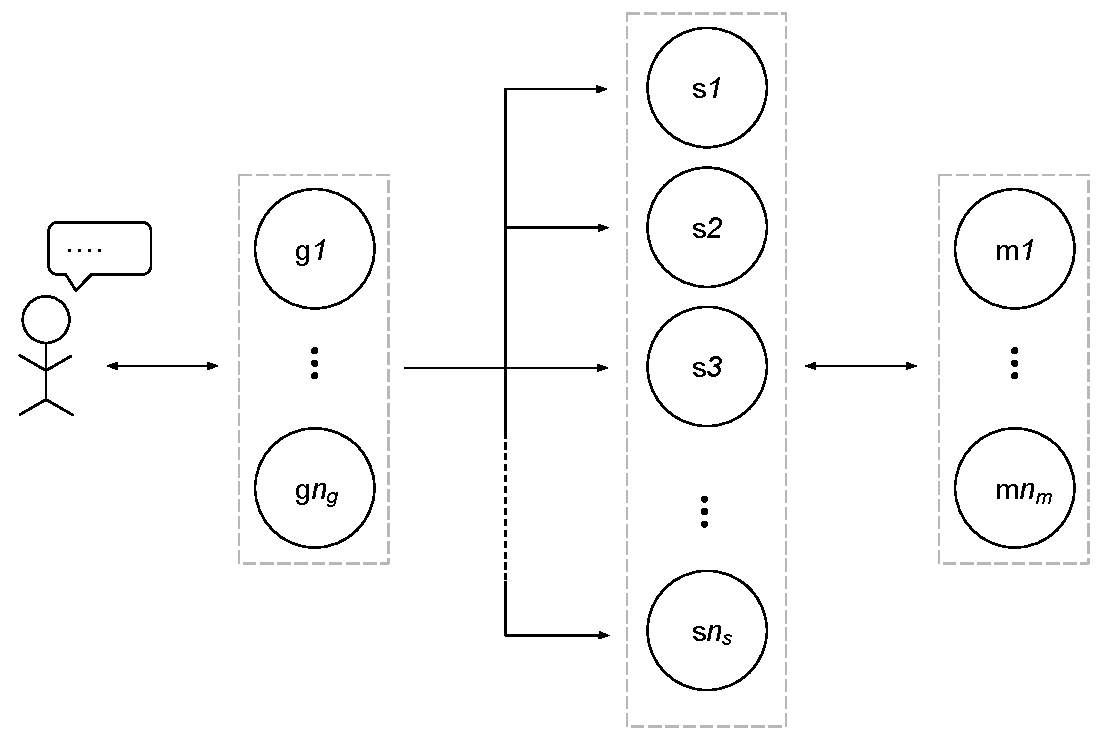
\includegraphics[scale=0.60]{pdf/sofa-overview.pdf}
	\caption[General overview of \CodeName]{General overview of \CodeName and the participating components and their associates, including $n_g$ gateways denoted by $\text{g}1 \ldots \text{g}n_g$, $n_s$ storage nodes by $\text{s}1 \ldots \text{s}n_s$ and $n_m$ monitors by $\text{m}1 \ldots \text{m}n_m$. \label{fig:sofa-overview}}
\end{figure}

\section{Overview}
This project is an alternative to the existing file archives targeting big data analysis frameworks; the architectural structure will be influenced and inspired by those described in related work (Section \ref{sec:related}), both by characteristics and feature, but certainly from inaccuracies too. 
\newline

The architecture of the file archive seeks to model an interpretation of a storage area network (SAN) primarily used for research and scientific related big data analysis, operating in a trusted homogeneous computing environment. The illustration at Figure \ref{fig:sofa-overview} depicts the general overview and flow of the system just described, where each component is examined subsequently in Chapter \ref{chp:components}.

\section{Hardware} \label{sec:hardware}
The framework is designed first and foremost to execute on a homogeneous collection of machines connected to a network such as a cluster, but the choice could have been a grid (a collection of heterogeneous machines) too. 
\newline

The implementation will be targeted inexpensive commodity hardware like Dynamo or the Google File System (Section \ref{sec:related}) and will be assembled by JBODs (Defintion \ref{def:jbod}) for this first version.

\vspace*{3mm}
\begin{definition}[JBOD] \label{def:jbod}
\textit{It is an acronym for Just a Bunch of Disks and is a hardware architecture with multiple hard drives, but without configuration of RAID and thus doesn't provide redundancy nor performance improvements.}
\end{definition}

The fact that the underlying component is a file archive related system built by bricks (Definition \ref{def:brick}) make clusters an obvious choice for a prototype.

\vspace*{3mm}
\begin{definition}[Brick] \label{def:brick}
\textit{A brick is defined as a component of a homogeneous distributed system, where each of them is functional equivalent and are contributing uniformly and have equal rights.}
\end{definition}
\vspace*{3mm}

\section{Architectural style} \label{sec:architectural-style}
The overall architecture of the project will be affected by knowledge and benefits from existing solutions (Section \ref{sec:related}) along with the theoretical background knowledge acquired by Tanenbaum \etal's description of distributed system architectures\cite{Tanenbaum:2006:DSP:1202502}. 
\newline

The result will seek to model the notion of a hybrid related distributed system with a decentralized collection of interconnected peer-to-peer storage nodes accessible by potentially multiple replicated stateless gateway servers and observed by one or more monitors.

\begin{figure}[h!]
	\centering
	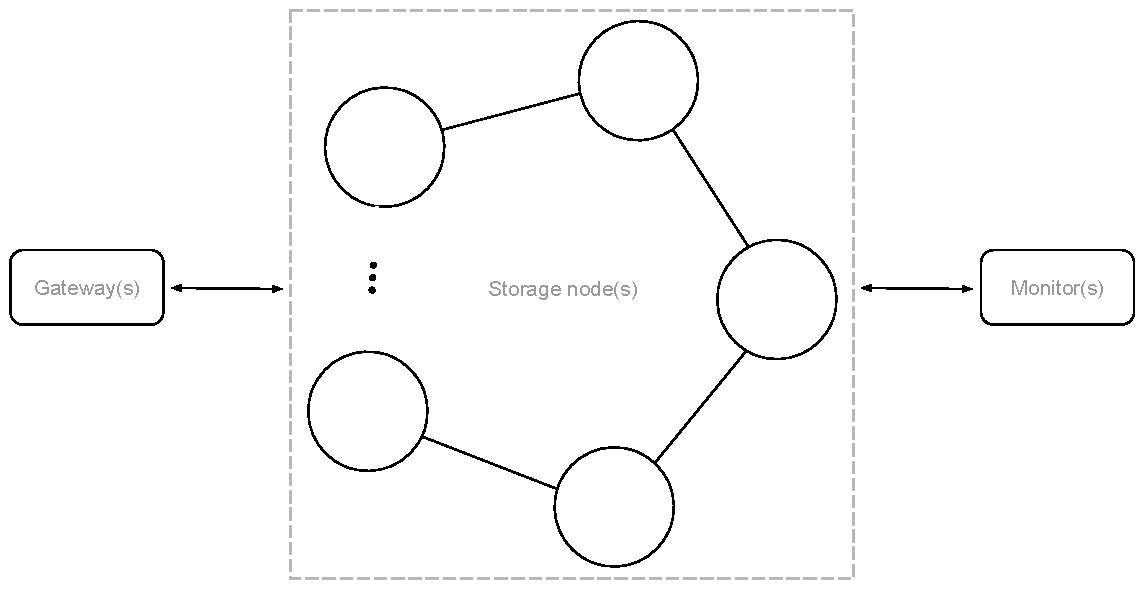
\includegraphics[scale=0.7]{pdf/architecture-overview.pdf}
	\caption[Architectural overview]{Architectural overview of the hybrid related distributed system reflecting a zero-hop distributed hash table ring of storage nodes. \label{fig:architecture-overview}}
\end{figure}

The architecture of the interconnected storage nodes (Figure \ref{fig:architecture-overview}) is highly influenced by Dynamo and will reflect a zero-hop distributed hash table (Definition \ref{def:dht}) and thus provides full data consistency concerning the CAP theorem (Definition \ref{def:cap}). Unfortunately, this also means that complexity regarding the consistency protocol increases at a membership protocol level.
\newline

The design and structure of the storage node will be described as part of Chapter \ref{chp:nodes} in Section \ref{sec:storage}, the gateway in Section \ref{sec:gateway} and the monitor in Section \ref{sec:monitor}.
\newpage

\begin{definition}[Distributed Hash Table] \label{def:dht}
\textit{DHT is undoubtedly the most-used organized peer-to-peer overlay network infrastructure, a procedure to arrange processes/nodes and links between them. Each node is assigned a unique identifier and a sub key-space\footnote{The available identifiers between two neighbor nodes}  generated by special hash-function, defined for that particular system and thereby placed onto the ring. Figure \ref{fig:dht} illustrates an example of a DHT ring.}

\begin{figure}[h!]
	\centering
	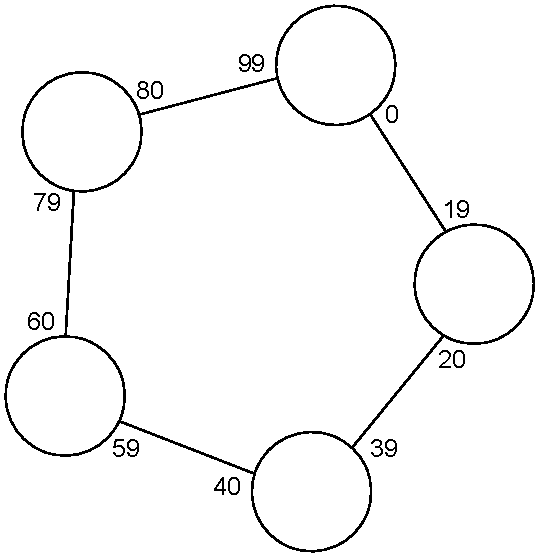
\includegraphics[scale=0.6]{pdf/dht.pdf}
	\vspace*{3mm}
	\caption[]{Example of a distributed hash table example with a key-space size of 100 and 5 storage nodes available. \label{fig:dht}}
\end{figure}
\end{definition}

\section{Communication} \label{sec:communication}
%TODO 

\section{Partitioning and distribution} \label{sec:pandd}
The partitioning and distribution protocol in \CodeName is based on consistent hashing (\reference{def:ch}{sec:partitioning}) and the round-robin load balancing algorithm (Definition \ref{def:rr}). The downside of this distribution algorithm is that it does not take state, availability and workload among other properties of the servers into account. 
\newline

However, this should be adequate assuming data is large enough and the framework primarily is expected to be operating in homogeneous and high-performance computing environment like a cluster (Section \ref{sec:presumptions}). Furthermore, one of the assumptions (Section \ref{sec:assumption}) is to implement a transparent but suitable load balancing protocol with big data analysis in mind.
\vspace*{3mm}

\begin{definition}[Round-robin] \label{def:rr}
\textit{A simple, fair share and starvation free load balancing algorithm that is easy to implement. The algorithm is distributing elements until there are no more among the available servers in a one-by-one or chunk-by-chunk fashion, thus the name of the algorithm.}
\end{definition}
\vspace*{3mm}

\begin{figure}[h!]
	\centering
	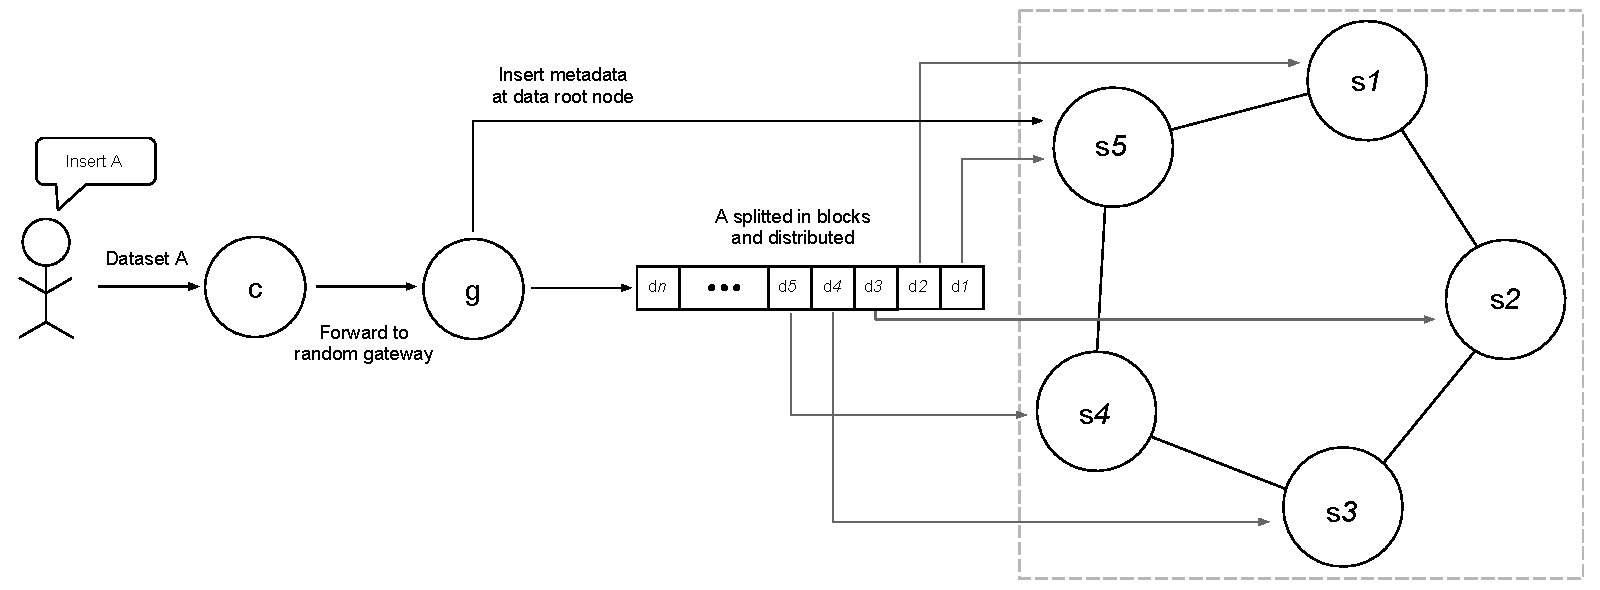
\includegraphics[scale=0.5]{pdf/rr-partitioning.pdf}
	\caption[Overview of the partitioning and data distribution protocol]{General flow of the partitioning and data distribution protocol in \CodeName, assuming one gateway server \textit{g} and a client \textit{c} attempting to insert data \textit{A} consisting of \textit{n} blocks $\text{d}1 \ldots \text{d}n$.\label{fig:rr-partitioning}}
\end{figure}

Figure \ref{fig:rr-partitioning} illustrates the general flow of the preferred partitioning and distribution protocol. The data is distributed from the client to an arbitrary gateway server, where it is assigned a unique identifier using consistent hashing (as in Amazons Dynamo project) and partitioned into approximately\footnote{As described in section \ref{sec:objectives} is one of the ambitions to store arbitrary sized block.} equal block sizes. The blocks are distributed in a round-robin fashion to the storage nodes, after the metadata for the data is assigned to the root server\footnote{The server responsible for the data, which is determined by the identifier.}.

\section{Naming and virtualization} \label{sec:virtualization}
A requirement is that each instance of \CodeNameFull is associated with a specific global instance name (Section \ref{sec:configuration}) \eg based on the research area or even specific data types. This name is predominantly used to virtualize components, data, and caches and thereby supporting multiple executions of \CodeName instances at once, with own domains.
\newline

Elements in the framework are identified using a structured naming based technique\cite{Tanenbaum:2006:DSP:1202502}, where each semicolon denotes an explicit and more specific context. 

\subsubsection*{Nodes}
The pattern of the naming scheme of node components (depicted at as a general overview at Figure \ref{fig:sofa-overview} and described in Chapter \ref{chp:nodes}) are characterized as following:
\begin{equation*}
	\texttt{sofa}:<\text{instance name}>:<\text{type ref}>:<\text{sequence number}>
\end{equation*}
, where \texttt{type ref} is one of following component types: gateway, storage or monitor and the \texttt{sequence number} is a positive increasing number in range $0\ldots n$ where $n$ is either the number of gateways, storage nodes or monitors respectively.

\subsubsection*{Data}
\begin{equation*}
	<\text{instance name}>:<\text{data type}>:<\text{data name}>
\end{equation*}

The naming scheme of data (Chapter \ref{chp:components}) are defined as above, where \texttt{instance name} is the same as above, the \texttt{data type} is an optional parameter if the framework supports multiple types. The name of the data is required to be unique and specified as \texttt{data name}. The \texttt{sofa} identifier is not necessary since the data is only accessible in a sofa based context.

\section{Redundancy and replication}
Redundancy in \CodeName is carried out using \eg software RAID-Z in ZFS (Description \ref{def:zfs}), which provides block-level striping with double distributed parity, that ensures fault tolerance by upto two failed drives. The motivation for this is that the existing replication protocols in \eg Hadoop and Google File System (Section \ref{sec:related} and \ref{sec:replication}) are using a vast amount of space and communication are too expensive considering that the primary usage of this is big datasets.
\newline

If the redundancy protocol however is based on erasure codes then it is no longer replication, but fault tolerance with a degree of durability. This type of responsibility is in this system carried out in hardware by the JBODs, such that there is no need for the extensive amount of network data transfer.

\begin{definition}[ZFS] \label{def:zfs}
\textit{It is composed of one or more virtual storage pools which are a collection of virtual devices that can be interpreted as a RAID (Redundant Array of Independent Disks) set in a standard file system.}
\newline

\textit{ZFS is an extensive 128-bit addressable file system that always is consistent on disk, this is because it performs a copy on write operation when adding new data, \ie writing modified data into a new space and reuse the old space in the future, thus eliminating the write hole error (corrupted file system) \eg on power loss.}
\end{definition}

\section{Recovery} \label{sec:recovery}
The RAID-Z configuration described in the previous section with the purpose of replication are also used as a basic recovery protocol to conceal disk failures. A second recovery initiative is redundant multipaths to efficiently hide server error.
\newline

The system will run on economical low-cost hardware such as JBODs (Definition \ref{def:jbod}) as explained in section \ref{sec:hardware}. Having SAS-controlled\footnote{Serial Attached SCSI: serial point-to-point protocol for moving data} disks enables fail-over features such as multipathing (Definition \ref{def:multipath}) that allows redundant data paths between host servers and the block-level devices.

\begin{figure}[h!]
	\vspace*{3mm}
	\centering
	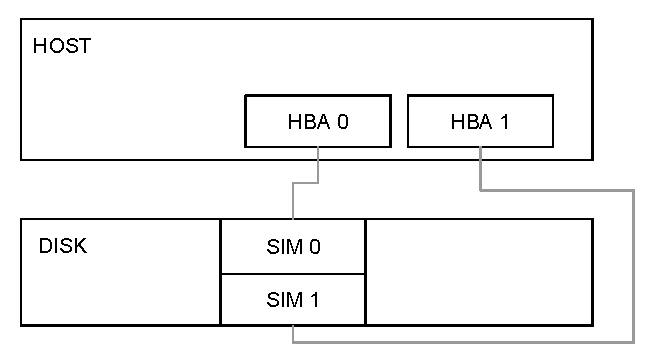
\includegraphics[scale=1]{pdf/1host-1disk.pdf}
	\vspace*{3mm}	
	\caption[Simple JBod setup]{JBod setup with one host and one array of disks.\label{fig:1host-1disk}}
\end{figure}
\newpage

Figure \ref{fig:1host-1disk} illustrates a simple example with one host and one array of disks, where:
\begin{itemize}
	\item \textbf{HBA} (Host Bus Adapter) is the local controller on the computer that connects it to other storage or network devices.
	\item \textbf{SIM} (SAS Interface Module) is the storage device controller.
\end{itemize}

Figure \ref{fig:2host-2disk} includes another more complex example to show the scalability with multiple hosts and disks.
\begin{figure}[h!]
	\centering
	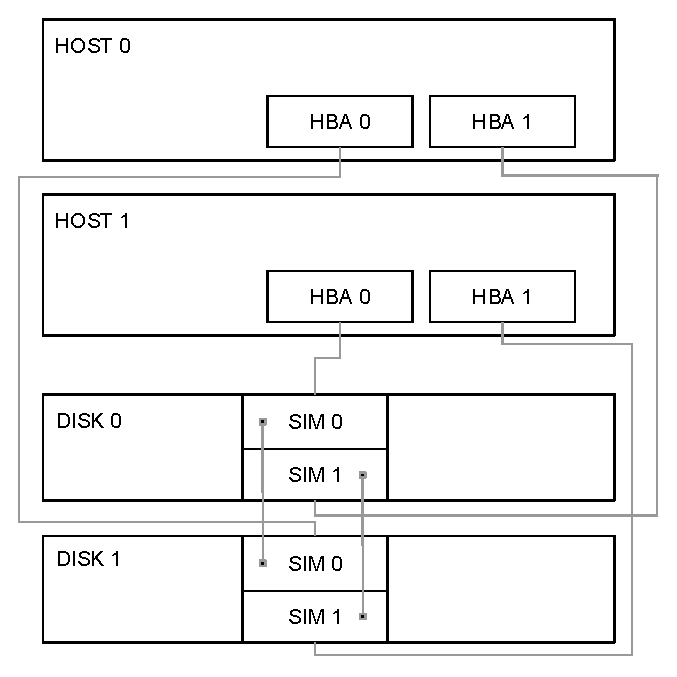
\includegraphics[scale=1]{pdf/2host-2disk.pdf}
	\caption[Complex JBod setup]{JBod setup with multiple hosts and multiple disks. \label{fig:2host-2disk}}
\end{figure}

\begin{definition}[DM Multipath] \label{def:multipath}
\textit{Multipathing is a Linux operating system device mapper for SAS-controlled hard drives that provides I/O fail-over and load balancing, by having numerous paths between host and disk. The configuration of DM Multipath is handled at an operating system level and the device controllers on the storage disks is unaware of such configurations.}
\end{definition}

\section{Security} \label{sec:security}
The focus on data integrity and security have predominantly been given low priority, since the system is expected to execute in a trusted environment, exactly like Amazon Dynamo, thus it is intentionally implemented without internal authentication or authorization.
\newline

Nevertheless, security is evidently an influential component and property at the boundary of the system, one of many actions is \eg using the secure HTTPS connection on the network requests to the entry gateway servers instead of ordinary HTTP. Validation of user input is most certainly also a reasonable action when it comes to security.


\chapter{Components} \label{chp:components}
Essential components of the \CodeName ecosystem will be described and discussed in the following chapter, which includes the core configuration of the system, such as accessibility and mounting points. Other essential components counts; the three nodes (Gateway, Storage and Monitor) mentioned in the Architecture and Design chapter and the foundation package including the \texttt{SofaBaseObject} and the operation context definition.

\section{System configuration} \label{sec:configuration}
Each instance of \CodeName running is specified by a set of different parameters in the configuration file. All parameters are chosen, defined and implemented in order to make each version as customizable as possible. Figure \ref{fig:cfg_example} is an example of a custom implementation of a \CodeName configuration.
\newline

Each configuration specification is written in a \texttt{.cfg} file format (explained in definition \ref{def:cfg})) with four predefined groups:
\begin{itemize}
	\item \textbf{general}: Used to define various thresholds, retries, and path, but most important the \texttt{instance-name} which differentiates this instance from the rest. Additionally, it enables virtualization (described in section \ref{sec:virtualization}) and recovery (described in section \ref{sec:recovery}).
	\item \textbf{gateway/storage/monitor}: Used to specify the addresses and pots of the three different nodes booted at startup.
\end{itemize}

The language chosen could have been YAML \cite{PageYaml} or even JSON, but the readability and white space insensitivity of config files was preferred.

\begin{figure}
\vspace*{4mm}
\begin{lstlisting}[language=bash, frame=single, basicstyle=\ttfamily\tiny, otherkeywords={[,],=}, numbers=none, deletekeywords=enable]
[general]
project-path = /code/sofa-project/sofa
log-file = /code/sofa-project/sofa.log
keyspace-size = 2**5
mount-point = /mnt/sofa/
instance-name = exampledata

# Defined in seconds
heartbeat-scheduler-delay = 1
num-heartbeat-retries = 5
enable-live-software-reboot = True

load-balancing-threshold = 1

# Defined in megabytes
block-size = 5.0

[gateway]
addresses = localhost:9999

[storage]
addresses = localhost:8888

[monitor]
addresses = localhost:7777
\end{lstlisting}

\caption{Example of a \CodeName configuration implementation \label{fig:cfg_example}}
\end{figure}

\vspace*{4mm}
\begin{definition}[.cfg] \label{def:cfg}
\textit{A commonly used generic preference file for parameters and initial settings for an application, which is defined in a flat text file format, with minor syntactic features such as groups.}
\end{definition}
\vspace*{6mm}

It is important to notice that the \texttt{block-size} parameter defines that maximum allowed size for any given block of data and not a fixed size for each, as this would violate following objective described in section \ref{sec:objectives}:

\begin{quotation}
	\textit{"To store data in arbitrary sized chunks as a consequence of above mentioned."}
\end{quotation}

Other configuration parameters such as \texttt{heartbeat-scheduler-delay} and \texttt{enable\-live-software-reboot} will be described and deliberated on as part of the components they strengthen.

\section{Storage node} \label{sec:storage}
% TODO: Menition Real-time scalable access model: NameService due to on the fly calculation of ids on all storage nodes

\section{Gateway} \label{sec:gateway}

\section{Monitor} \label{sec:monitor}
% TODO: Reference to \ref{sec:recovery} from architecture when writing about live software reboot - also reference to the system configuration \ref{sec:configuration}

\section{Delegation} \label{sec:delegation}
% TODO: Reference to \ref{sec:recovery} and DM Multipath as load balancing together with load-balancing-threshold in the forward queue

\newpage

\section{\texttt{SofaBaseObject}} \label{sec:sofabaseobject}
Dataset in \CodeName has to adhere the interface defined in the \texttt{SofaBaseObject}, which is composed and designed in such a way that the associated data potentially\footnote{Vastly depended on how the function from the interface is implemented.} is stored and processed optimally.

\vspace*{5mm}
A dataset is defined by a number of properties:
\begin{itemize}
	\item A unique \textbf{name} that will be used to identify it, throughout the lifetime of the dataset in \CodeName.
	\item An optional \textbf{description} parameter to differentiate between and recognize dataset with similar or ambiguous names.
	\item Optional list of \textbf{operation context}s (described subsequently in section \ref{sec:operation} in this chapter) to be executed on the data.
\end{itemize}
\vspace*{5mm}

, and a number of required, and optional functions that will be discussed and described in details throughout the rest of this section since it is crucial to understand how, what seems like a limiting amount of functions, is general and generic enough to describe any type of data and operations to be executed on it. The meaning of the term \textit{operation (context)} and the purpose will be described subsequently in this chapter in section \ref{sec:operation}. 
\newline

Figure \ref{fig:preprocess-nextentry} illustrates the context of which following required and optional functions: \textbf{preprocessing}, \textbf{next entry}, \textbf{replication factor} and \textbf{distribution strategy} are used in the flow of adding new data (the append API\footnote{Application Programming Interface} will be described in chapter \ref{chp:api}).

\begin{figure}
	\centering
	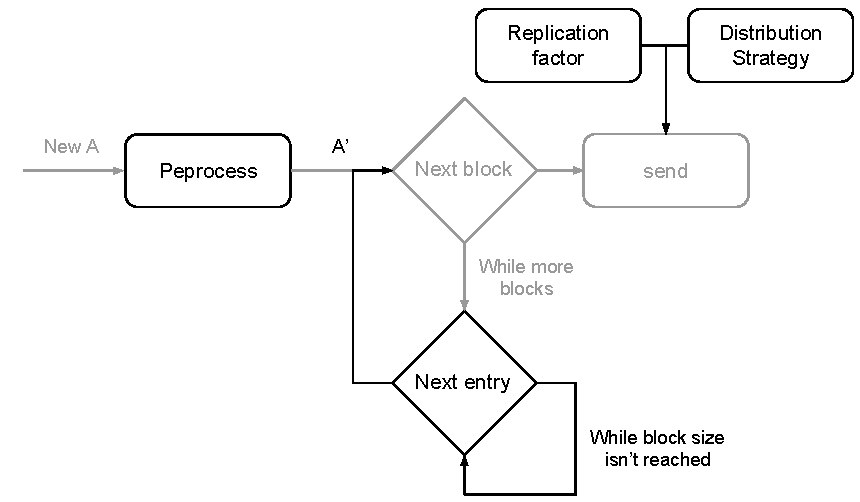
\includegraphics[scale=0.8]{pdf/preprocess-nextentry.pdf}
	\caption[\texttt{SofaBaseObject} interface functions]{Illustration of where some of the \texttt{SofaBaseObject} interface functions are used. The ones depicted in a light shade of gray are other key parts of the append operation that will be described later in chapter \ref{chp:api}: Core API. \label{fig:preprocess-nextentry}}
\end{figure}	

\subsection{Prepossessing}
A step that is executed initially when new data is added to \CodeName before it is split. This step facilitates options\footnote{Built-in \CodeName function to load data from local path or url are provided and accessible through the \texttt{SofaBaseObject} API.} such as reshaping data array if they are fetched over network or loading the data as a specific object type.

\subsection{Next entry}
The purpose of this function is to transition the responsibility of split the data correctly towards the end-user, rather than imperfection choices by the system. With this approach, \CodeName relies on the users know-how and expertise regarding the internal structure of the data and how to split it semantically correct, such that coherent parts are jointly stored.
\newline

The consideration and complexity behind this required function and its role as part of the append-flow (depicted in figure \ref{fig:preprocess-nextentry}) jointly contribute to a generic solution that optimally will accomplish following objective described in section \ref{sec:objectives}: 

\begin{quotation}
	\textit{"Split data such that semantically coherent parts are stored jointly and thus eliminating the data residual problem known from Hadoop."}
\end{quotation}
\vspace*{3mm}

While the users now have been granted some, not unreasonable responsibilities are \CodeName on the other hand in control of combining semantic blocks and distributing them concerning the distribution strategy and replication factor.

\subsection{Distribution strategy}
\CodeName provides three different distribution strategies for the semantic blocks, the strategies are offered at a data level and not at a system wide level as in many other alternatives, such that it can be tailored ideally to each specific use-case. The three ones are:

\begin{enumerate}
	\item \textbf{1-by-1}: A basic implementation of the Round Robin distribution and scheduling algorithm (outlined in definition \ref{def:rr}).
	\item \textbf{Tiles}: Extended version of the Round Robin algorithm with support for \textit{n}-by-1, such that semantic blocks are tiled/grouped by \textit{n} before distribution.
	\item \textbf{Linear}: A specific single run-through version of the tiles strategy algorithm described above, where the blocks are distributed as equally as possible\footnote{ Eq: $\lceil blocks / storage\_nodes\rceil$, to make sure that there isn't an overabundant of blocks on last server (\CodeNameShort's interpretation of \textit{'last'} server will be explained subsequently in chapter \ref{chp:api}).} across the storage nodes.
\end{enumerate}
\vspace*{5mm}

\begin{figure}[ht!]
	\centering
	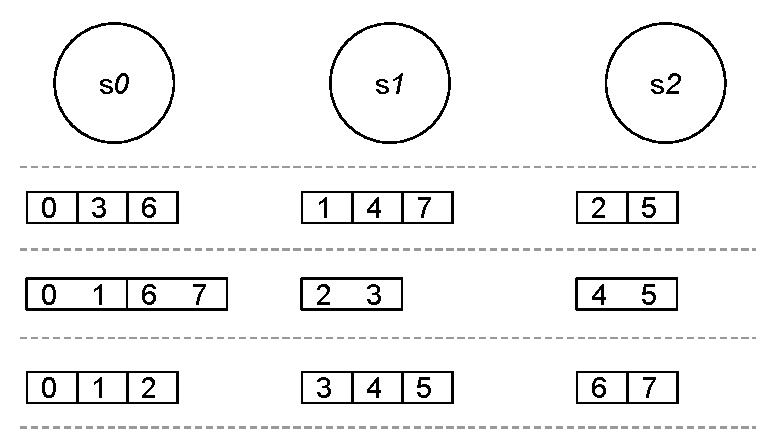
\includegraphics[scale=0.85]{pdf/distribution-strategies.pdf}
	\vspace*{3mm}
	\caption[Distribution strategies]{An Example of how the three distribution strategies work in action. The figure illustrates three storage nodes denoted by s\textit{0}, s\textit{1} and s\textit{2} and the block stored on them with strategies of respectively \textbf{1-by-1}, \textbf{Tiles} of size 2 and \textbf{Linear}. \label{fig:distribution-strategies}}
\end{figure}	

It is worth to notice that all the different distribution strategies in one or another way are a variant of the Round Robin algorithm and thereby adhere to the architecture and design criterion for partitioning and distribution described in section \ref{sec:pandd}.
\newline

Although the strategies initially appear to be approximately equal, the results of appending eight blocks on three storage nodes are very divergent (result depicted in figure \ref{fig:distribution-strategies}) and thus one could easily find very different purposes for each:

\begin{quotation}
Data with an extensive interrelationship between blocks are a straightforward example of where a tiled strategy would be preferable, since operations on such data usually would require a considerable amount of exchanges of ghost points with the neighbors (a technique Wilkinson \etal covers in \cite{Wilkinson:1998:PPT:289352} and that will be explained in section \ref{sec:operation}) to produce the expected results. Even though a linear distribution strategy also would work for this purpose, it is a requirement that the total number of blocks are known on beforehand, since data is streamed into \CodeName.
\end{quotation}

One could think of other distribution strategies and algorithms to use on certain specific types of data, hence its an ambition subsequently to design and come up with a generic interface for defining individual strategies and algorithms.

\subsection{Replication}
\CodeName provides the opportunity of virtual replication at a data level specified independently for each dataset. Compared to other alternatives as the ones evaluated in section \ref{sec:related} such as Hadoop this is a unique and contemporary privilege, since replication commonly is at a machine level. Preceding enables options for prioritizing datasets with regards to importance and reproducibility of data.
\newline

The replication factor can additionally be used as a load balancing mechanism for the dataset and thereby increase its accessibility for the end-users, this among other things were described and discussed in section \ref{sec:delegation}.

%\subsection{Verification}
%In \CodeNameShort, verification of individual operation context functions\footnote{An operation context is assembled by one or more functions, this will be described in details in section \ref{sec:operation}).} is required when utilizing the optional list of operation contexts parameter. In order 

\section{Operation context} \label{sec:operation}
An \texttt{OperationContext} is a mutable object attached to a dataset that represents and describes a function or multiple chained ones and the associated parameters and prerequisites, to be executed on the data. A number of optional specifications are available such that most most common requirements are supported out of the box to increase productivity and correctness.
\newline

The syntax for characterizing this object, the optional specifications, and a lot more will be examined in details throughout the rest of this section since it is crucial to understand too, like the other foundation object \texttt{SofaBaseObject} described in section \ref{sec:sofabaseobject}.

\subsection{Sequential / Parallel}
Functions of an operational context can be grouped in an unlimited amount of nested sequential and parallel containers, although it is required that the outer most container is of the sequential type. The two code snippets in the forthcoming \textbf{syntax} sections exemplifies the usage of these two varies.

\subsection{Syntax}
The \texttt{OperationContext} object can be instantiated in two ways depending on the end-users preferences:
\vspace*{2mm}

\begin{enumerate}
	\item In a traditional fashion way:
\vspace*{2mm}
\begin{lstlisting}[language=Python, basicstyle=\footnotesize, numbers=none, showtabs=false, showstringspaces=false, showspaces=false, 
otherkeywords={[,{,},],Sequential,Parallel,OperationContext}, deletendkeywords={sum}]
OperationContext(Sequential(Parallel(
                            Sequential(count, sum), 
                            Sequential(count_nocase, sum)
                           ), equality))
\end{lstlisting}
\vspace*{-2mm}
	\item And the effective customizable shorthand version:
\vspace*{2mm}
\begin{lstlisting}[language=Python, basicstyle=\footnotesize, numbers=none, showtabs=false, showstringspaces=false, showspaces=false, 
otherkeywords={[,{,},],Sequential,Parallel,OperationContext}, deletendkeywords={sum}]
OperationContext.by('[{[count, sum], 
                       [count_nocase, sum]
                      }, equality]')
\end{lstlisting}
\vspace*{-2mm}
	The sequential (\texttt{[} and \texttt{]}) and parallel operators (\texttt{\{} and \texttt{\}}) are the default ones but are changeable as long as they all four are distinct and aren't string definition syntax operators, such as \texttt{'} and \texttt{"} as in most common programming languages.
\end{enumerate}

\subsection{Ghosts}
In \cite{Wilkinson:1998:PPT:289352} Wilkinson \etal covers the technique of ghost points which is a procedure well studied and used in high performance computing, etc. Common computing challenges where this is superior are typically situations where the data has an immense correlation between the semantic blocks such as image data or climate simulation results, as previously described. 
\newline

Figure \ref{fig:ghost-points} illustrates the fundamental idea behind ghost points also denoted as halo lines where each domain has an extra row of data added at the boundary between the others consisting of data from the neighbor. 

\begin{figure}[ht!]
	\centering
	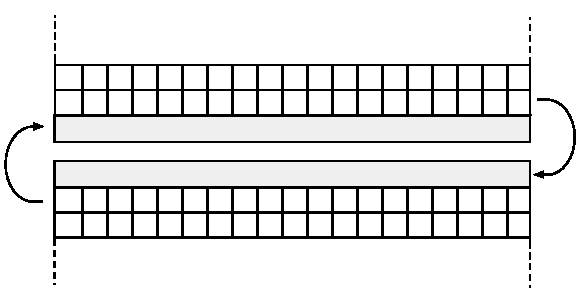
\includegraphics[scale=0.92]{pdf/ghost-points.pdf}
	\vspace*{3mm}
	\caption{Fundamental idea of ghost points \label{fig:ghost-points}}
	\vspace{2mm}
\end{figure}	

One or more rows are exchanged between neighbors in order to compute the accurate results beyond everything, but also to minimize the I/O-cost compared to exchanging data independently when needed.
\newline

\begin{figure}[ht!]
\centering
\vspace*{6mm}
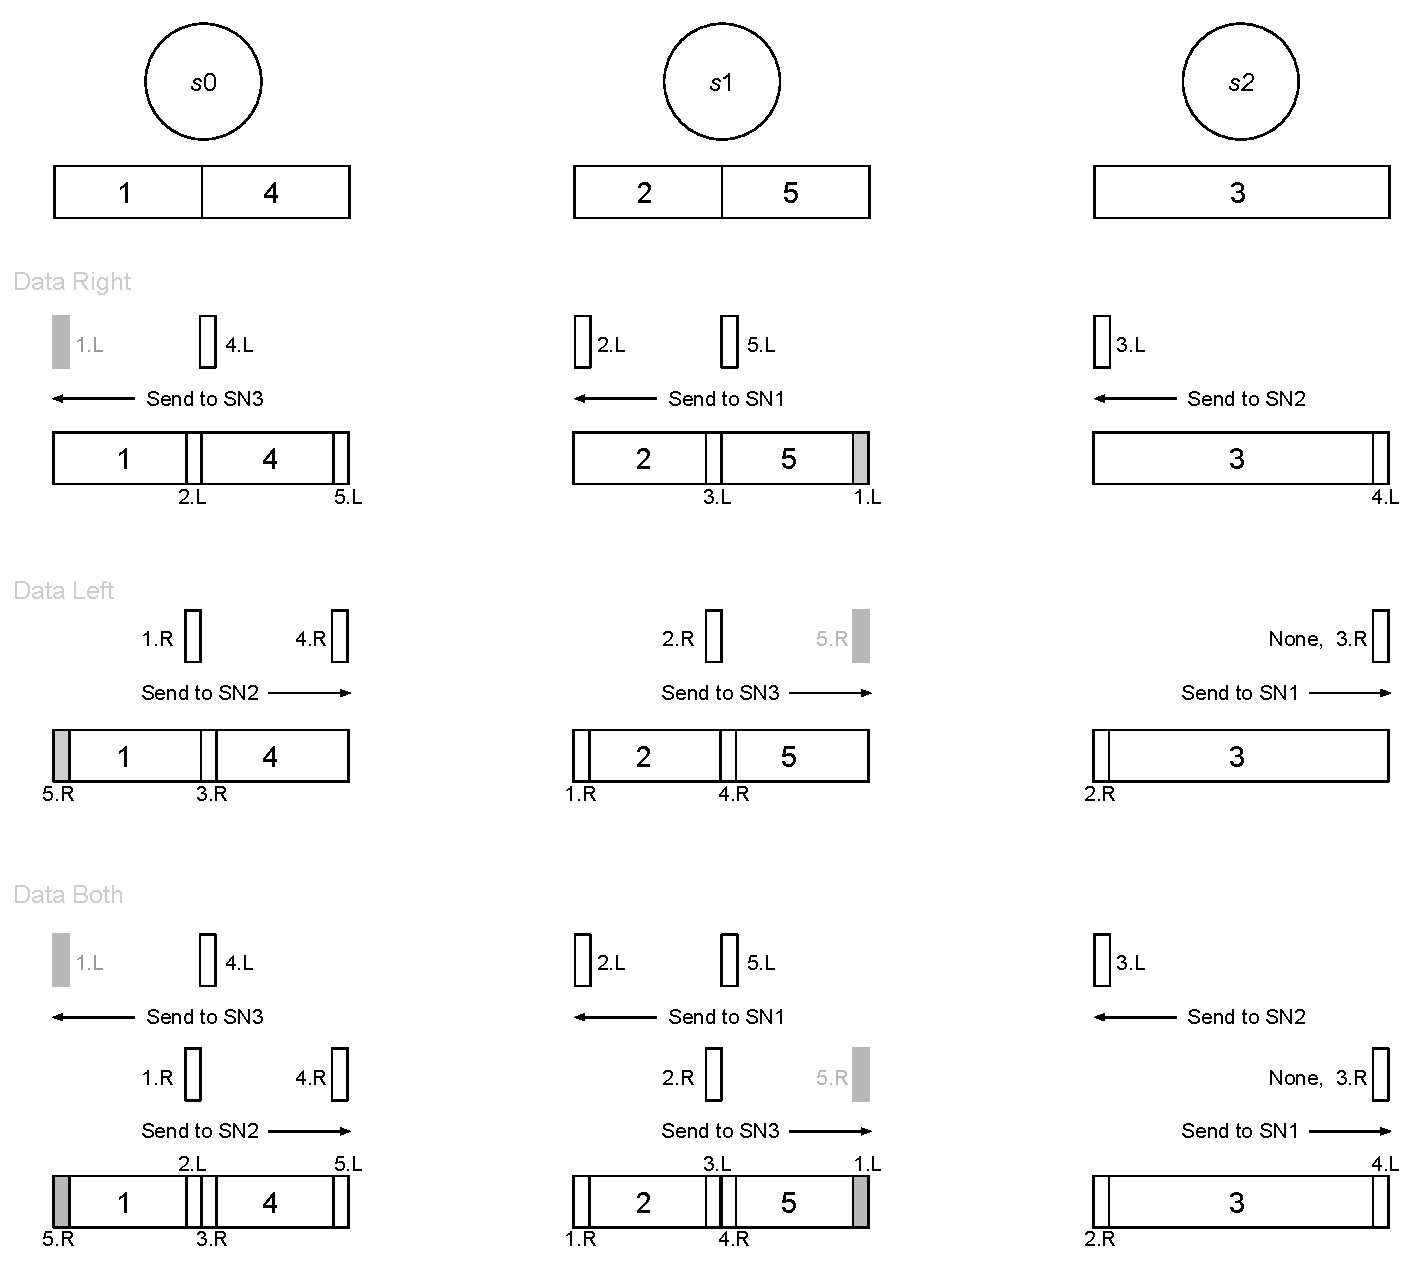
\includegraphics[scale=0.55]{pdf/ghost-transfer.pdf}
\vspace*{4mm}
\caption[Ghost transfer example]{Example of how ghost points are transferred between nodes.}
\vspace*{6mm}
\label{fig:ghost-transfer}
\end{figure}

Figure \ref{fig:ghost-transfer} illustrates the flow of the three supported types of ghost point exchange in \CodeName:

\begin{enumerate}
	\item Sending data clockwise / \textbf{right}.
	\item Sending data counterclockwise / \textbf{left}.
	\item And in \textbf{both} directions with symmetric and asymmetric semantic units as ghosts.
\end{enumerate}
\vspace*{2mm}
, though, there is a limitation held in common by all three of them; that data \textbf{overflow} from first to last when transferring left and last to first when transferring right aren't implemented for the time being.
\newline

The neighbor exchange protocol is implement by default in \CodeName and can be utilized in two different ways:

\begin{enumerate}
	\item As a \textbf{preprocessing} step for operations where ghosts are demanded initially.
	\item Moreover, as a built-in keyword function\footnote{Defined and explained later in this section.} used as an intermediate step before a function requiring ghosts in the chain of functions.
\end{enumerate}

\subsubsection*{Protocol}
The naïve approach for implementing a ghost point distribution protocol using Figure \ref{fig:sofa-overview} as starting point is to:
\begin{enumerate}
	\item First of all, let the gateway initialize the process at the root node\footnote{The definition of a root node for a dataset was defined in section \ref{sec:storage} previously in this chapter} for that particular dataset.
	\item Moreover, let that node initialize the calculation and exchange protocol on all the nodes with segments of the data.
	\item Finally, every storage node ask every neighbor for their needs in terms of ghost semantic blocks.
\end{enumerate}
\vspace*{2mm}
Such procedure as explained above requires a minimum of $5n-1$ I/O requests which is rather suboptimal. In distributed systems the focus is on optimizing the number of those requests and one could easily think of an optimized solution such as the one illustrated at Figure \ref{fig:ghost-v1}. 

This solution, which improves number of initialization requests (from $n-1$ to $n/2-1$) among others, requires $\frac{5}{2}n-1$ I/O operations which is a remarkable improvement compared to the previous amount.

\begin{figure}[ht!]
	\centering
	\vspace*{3mm}
	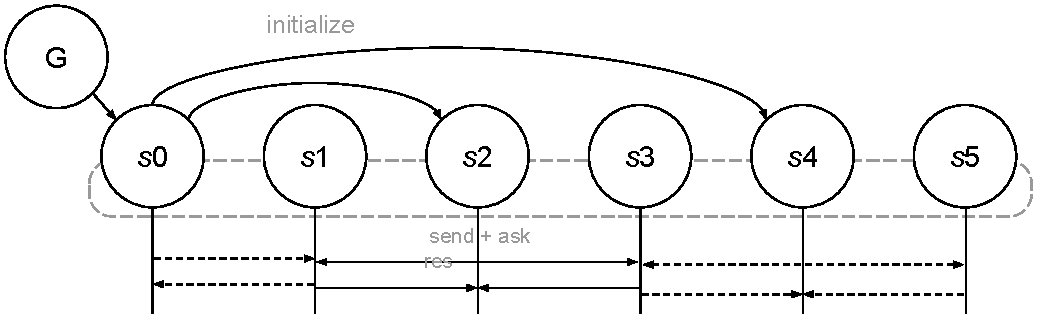
\includegraphics[scale=0.68]{pdf/ghost-v1.pdf}
	\caption{Ghost protocol v2: Initial design and thoughts \label{fig:ghost-v1}}
	\vspace*{3mm}
\end{figure}	

However, in high performance computing (HPC) clusters as this prototype framework first and foremost is targeted (as mentioned in section \ref{sec:hardware}) it is a matter of time steps and not I/O as such for which the HPC solution illustrated at Figure \ref{fig:ghost-final} is most optimal.
\newline

\begin{figure}
	\centering
	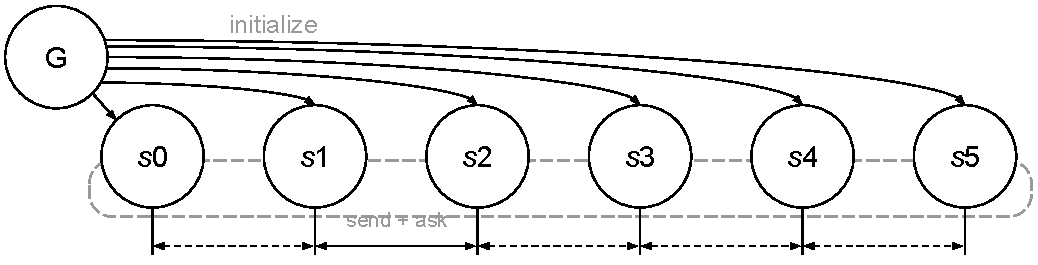
\includegraphics[scale=0.68]{pdf/ghost-final.pdf}
	\caption{Ghost protocol v3: The HPC solution \label{fig:ghost-final}}
\end{figure}	

This solution implements a \textit{"send fast, receive late"}-terminology based broadcast storms\footnote{Requires reasonable network and communication library implementation to be an improvement to prior solutions.} on the prior knowledge that every node knows what the two neighbors needs (regarding ghost semantic blocks), due to the scalable access model where all storage components at real-time can calculate others ids and thereby requirements. The broadcast storm is superior in highly synchronous environments like this where everybody can calculate and send at the same time and equivalently for receiving and thus utilizing the network bandwidth the most. 

\subsection{Postprocessing}
An optional step executed after the core of the operation has completed and before the end-user gets the result. This step facilitates options such as filtering or plotting data to produce quality figures on-the-fly at once.

\subsection{Built-in keywords}
\CodeName offers a range\footnote{Effortlessly extended when demanded} of different built-in keyword functions for conventional operations on data along with a module importer library that easily binds language specific core functions to \CodeName operations and functions, with a function name change if requested.

An example: \texttt{count(}x, y\texttt{)} is a built-in function from the \texttt{string} module in Python that counts number of \texttt{y} in \texttt{x}. Following snippet transforms the \texttt{count(}x, y\texttt{)} into \texttt{count\_occurrences(}x, y\texttt{)} with identical logic parameters and results:
\vspace*{2mm}
\begin{lstlisting}[language=Python, basicstyle=\footnotesize, numbers=none, showtabs=false, showstringspaces=false, showspaces=false, otherkeywords={string,new_fun_names}, stringstyle=\color{blue}]
   module_binder(string, function_binder, ['count'], 
                 new_fun_names=['count_occurrences'])
\end{lstlisting}

Noticeable keyword to discussed and elaborate on are:
\vspace*{2mm}

\begin{itemize}
	\item The \textbf{modify} keyword function takes one argument defined by a semicolon: \texttt{modify:<function\_name>} and calls the action defined by the \texttt{function\_name} parameter with the current data block state. The modify function is especially useful in combination with the module importer service since it is quite often that general core functions require that data to be in a certain format.
	\item \textbf{neighborhood} takes either zero, one or two arguments\footnote{Separated by a semicolon as for the other keyword functions.} and implements the ghost point transfer protocol described previously in this section.
	\begin{enumerate}
		\setcounter{enumi}{-1}
		\item \texttt{neighborhood}
		\item \texttt{neighborhood:ghost\_count}
		\item \texttt{neighborhood:left\_ghost\_count:right\_ghost\_count}
	\end{enumerate}
	The default value of \texttt{neighborhood} is \texttt{neighborhood:1}, which again is a equivalent to \texttt{neighborhood:1:1}. The function with two arguments mainly cohere asymmetric counts, \ie \texttt{left\_ghost\_count} $\neq$ \texttt{right\_ghost\_count}.
\end{itemize}


\chapter{Core API} \label{chp:api}
The core public API\footnote{Application Programming Interface} of \CodeName will be explained, demonstrated and documented in the following chapter. The routines defined, provides facilities to develop powerful and useful extensions and applications, through the minimal but adequate interface. Two examples of extensions empowered by the public \CodeName API are explained subsequently in part \ref{prt:extensions} and are demonstrations of the strength and confirms that all the building blocks needed are available.
\newline

The protocol exposes a vast amount of various \texttt{get}-methods to retrieve useful information regarding the datasets such as metadata, in addition to the routines explained in this chapter.

\section{General}
The formalities which are consistent throughout all of the routines are examined and described in this section.

The API is implemented in Python\cite{PagePython}, which is a high-productivity rather than high-performance programming language that have caught much attention and gained popularity in the high performance and research communities where the utilization thus has increased. The reason for the increased acceptance is because the language easily is extended by open source libraries written in other traditional high-performance languages like Fortran or C++, with a corresponding bridge such as Cython\cite{PageCPython} for C/C++. 
\newline

These types of bridges are are usually an optimising static compilers for Python that simplifies, and minimizes the hard work in the cross language integration. Examples of such library is the de-facto standard in scientific programming, NumPy \cite{PageNumpy} \cite{oliphant2006guide} that is implemented using Cython and Bohrium \cite{PageBohrium} \cite{kristensen2013bohrium} which is a runtime environment for efficiently executing vectorized code on a range of different hardware platforms\footnote{Such as CPU and GPU}.

\begin{quotation}
Python as the main programming language was chosen over others such as C++ and Java based primarily on its high-productivity and thus an appropriate prototype environment in addition to the integration abilities described above.
\end{quotation}

All communication in \CodeName between nodes and the public API is implemented using a Pyro4\cite{PagePyro4}, a remote procedure call library for Python that facilitates communication across the network by minimizing the workload. The library was chosen due to simplicity and precedence with regards to the project scope, but as mentioned in section \ref{sec:communication} there were other alternatives, which in a final solution potentially would increase performance.
\newline

The API seeks to implement a classic CRUD (Create, Read, Update and Delete) pattern with well-known slightly modifications, such as \textit{retrieve} instead of read in terms of the \texttt{get}-methods discussed and an extra \textit{append} functionality to attach data to the dataset.

\section{Create} \label{sec:api-create}
\CodeName provides a dynamic create API call for initializing new empty\footnote{With no data attached} datasets from a required unique name, a required Python class name and package reference like \texttt{example.data.MySpecialDataset} and an optional dictionary of specific extended user and dataset defined metadata attributes, apart from the private configuration \CodeName defined ones.
\newline

The anonymous unique identifier of a dataset is calculated by a hash function\footnote{A mapping function used to represent arbitrary sized data in a fixed space.} and is limited to the key-space size defined in the system configurations, described in details in section \ref{sec:configuration}, to find the responsible root node index (primary replica), which appended to the metadata of the dataset:
\begin{equation}
	\texttt{hash}:name \texttt{ mod } \texttt{\#}keyspace
\end{equation}

The concatenated package and class name are internally transformed to \CodeName \texttt{OperationContext} closure byte stream by compressing\footnote{Using the \texttt{marshall} \cite{PageMarshall} library which by \cite{Brody2015} is approximately 50\% faster than the regular \texttt{cPickle}.} it with an associated digest as a cryptographic signature. The closure is the core of operation execution in \CodeName, which will be explained further in details in section \ref{sec:submit}.

\begin{figure}[ht!]
	\centering
	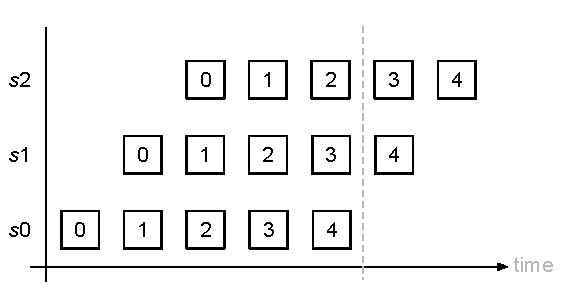
\includegraphics[scale=1.1]{pdf/package-pipeline.pdf}
	\caption{Timing diagram with example of package pipelining \label{fig:package-pipeline}}
\end{figure}	

\section{Append} \label{sec:api-append}
Whenever the frame for a dataset is initialized in \CodeName by the create call, it is possible to append data to it by either one of three ways: \textit{local path}, \textit{url} or \textit{true data}. The unique name that a dataset is initialized with is used whenever any of the other method calls such as \textit{append} or \textit{delete} are utilized. 
\newline

The append call implements the previous described important flow illustrated at Figure \ref{fig:preprocess-nextentry} and thus is the core of succeeding following two objectives (described in details in section \ref{sec:objectives}):

\begin{quotation}
	\textit{Split data such that semantically coherent parts are stored jointly and thus eliminating the data residual problem known from Hadoop.}
\end{quotation}
\noindent
and
\begin{quotation}
	\textit{To store data in arbitrary sized chunks as a consequence of above mentioned.}
\end{quotation}

The responsible dispatcher examined in section \ref{sec:delegation} and depicted at Figure \ref{fig:delegation-framework} is disabled for this particular call only, due to bandwidth rate and latency on transferring new data to a node not responsible for that semantic block of data first before redirected to the right one.

The gateway is for this call capable of determining the responsible server without relaxing excessively on the stateless property, by using the root index added to the metadata in the create-call, to calculate the primary replica index of a specific semantic block:

\vspace*{2mm}
\begin{equation} \label{eq:startindex}
	\Big\lfloor\Big(\texttt{id}:root + \dfrac{\texttt{\#}blocks}{stride}\Big) \texttt{ mod } \texttt{\#}storagenodes\Big\rfloor
\end{equation}

, where the \textit{stride} is a constant specific for each dataset and decided by the distribution strategy, described in section \ref{sec:sofabaseobject}.

\begin{quotation}
	{\sffamily\textbf{NOTE:}} As an aftermath of the abovementioned calculation in equation \ref{eq:startindex}, it is possible henceforth to pick up and append new data to dataset where it left off.
\end{quotation}

\subsubsection*{Package distribution}
Figure \ref{fig:package-pipeline} illustrates a suggestion to an ideal HPC package distribution solution for the append flow implementation, based on the common concept of pipeline computation that Wilkinson \etal describes in \cite{Wilkinson:1998:PPT:289352}. The model is designed to stream fragmented semantic block packages in a pipeline fashion between the gateway and the list of required replicas (as described in section \ref{sec:delegation}) in a priority queue.
\newline

The latency for streaming one package, assuming a network speed of 1 Mb/s and a fragmented package size of 1 MB is:
\begin{equation}
	\dfrac{\texttt{\#}fpackage}{network\text{ }speed} = \dfrac{8\cdot 1024^2 \text{ bits}}{1024^3 \text{ bits/s}} = \dfrac{1}{128} \text{ sec}
\end{equation}

, which with a replication factor of \textit{x} and an assuming total package size of maximum 64 MB (customisable in the system configurations) leads to a replication latency of:
\begin{equation}
	(64 + x - 1) \cdot \dfrac{1}{128} \text{ sec}
\end{equation}

, where the $x - 1$ directly can be derived from Figure \ref{fig:package-pipeline}, with the light gray, dotted line indicates when the first node has finished receiving and transmitting.
\newline

\noindent
Unfortunately, the fragmented package solution explained, requires the communication library applied to support streaming, which Pyro4 doesn't\footnote{Nevertheless, it was chosen based on the criteria and features listed previously.}. The package distribution algorithm implemented in \CodeName is based on the same technology and research as the protocol carried out in the delegation framework, namely the store and forward method. This also means that if the puzzle of replacing the communication library with a more suitable one, it will improve the delegation framework too.
\newline

Current implementation has following latency on sending one 64 MB semantic package and with the same network speed as the previous example:
\vspace*{1mm}
\begin{equation}
	\dfrac{\texttt{\#}package}{network\text{ }speed} = \dfrac{64\cdot 8\cdot 1024^2 \text{ bits}}{1024^3 \text{ bits/s}} = 0.5 \text{ sec}
\end{equation}
\vspace*{2mm}

\noindent
, and thus have a \textit{x} replication latency of:
\begin{equation}
	x \cdot 0.5 \text{ sec}
\end{equation}
 
\section{Update}
Based on the same logic as described in the create call (section \ref{sec:api-create}) but an initialized dataset is a prerequisite before it can be updated.

\section{Delete}
Remove an existing dataset and all associated semantic blocks and replicas, by its 	initiating name.

\section{Submit} \label{sec:submit}
Figure \ref{fig:submit-job} illustrates the bulk synchronous parallel like model implemented in the submit call. The request is forwarded to the responsible replica (described in section \ref{sec:delegation}) before initialization, which if needed is causing a parallel exchange of semantic ghost points (described in section \ref{sec:operation}) on the \textit{n} storage nodes. The interchange happens before the responsible server is initializing the parallel execution of the actual operation, which begins once the $n-1$ storage nodes have reported ready to the root node.
\newline

\begin{figure}
	\centering
	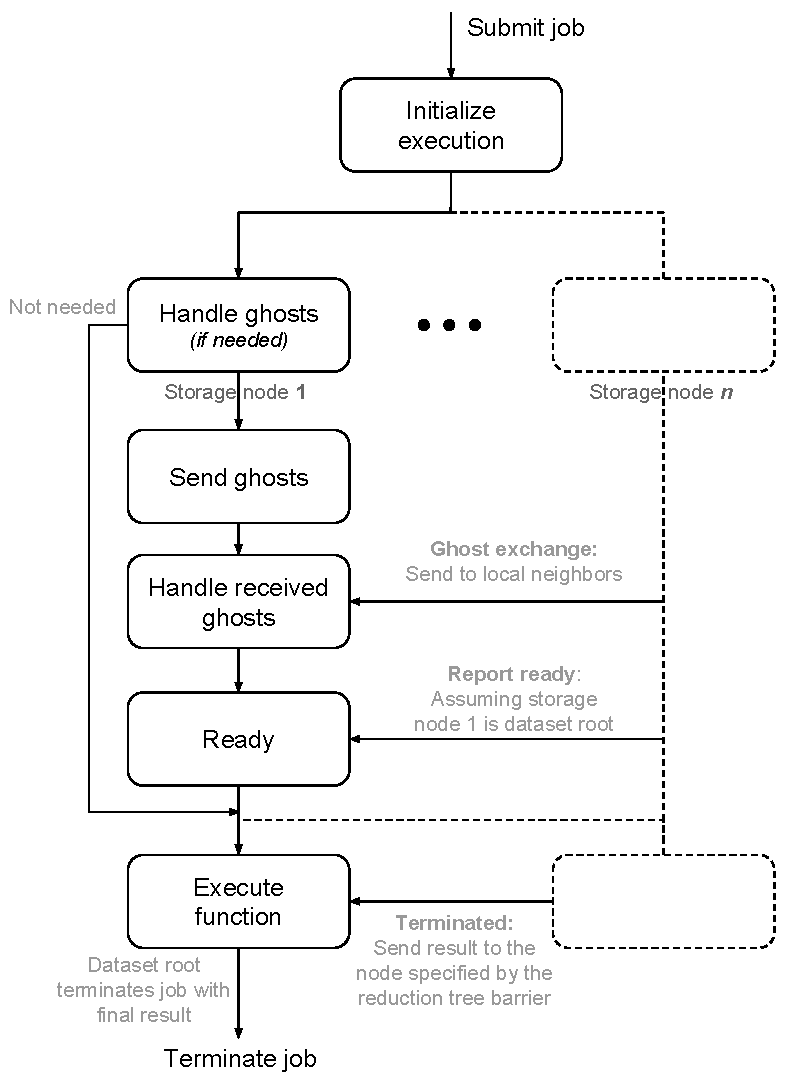
\includegraphics[scale=0.7]{pdf/submit-job.pdf}
	\caption{Flow diagram of the submit API call. \label{fig:submit-job}}
\end{figure}	

\noindent
The reason for the barrier before the execution is to ensure that all storage nodes is in charge of the data required for the calculation, such that no superfluous intercommunication is needed.
\newline

The execution of the operation itself is implemented as a tradeoff between minimizing I/O cost and reducing the load on the root node. The solution is based on the logic of the arrival part of a tree implementation of a barrier as illustrated in the example with 16 storage nodes at Figure \ref{fig:reduction-tree} and explained by Wilkinson \etal in \cite{Wilkinson:1998:PPT:289352}.

A solution particularly well-suited for big data analysis with MapReduce (outlined in definition \ref{def:mapreduce}) as primary data execution model, a statement that is clarified and explained in details with tangible examples in chapter \ref{chp:bdae}.
\newline

The calculation of whom to send to who is based on a multiplication of the \textit{sum of odd numbers}\footnote{$1 + 3 + 5 + \ldots + (2n-1) = n^2$} with respect to the iteration count (the x-axis at the figure). The calculation for any given iteration \textit{i} is as follows:
\begin{equation} \label{eq:reduction}
\underbrace{\dfrac{\texttt{id}:node}{2^{i}}}_{\forall \in \mathbb{N}_0} \texttt{ mod } 2 \equiv 1
\end{equation}
, and will resolve in boolean values that indicate whether the node has to send its result to the closest neighbor on the left-hand side.
\newline

\begin{figure}
	\centering
	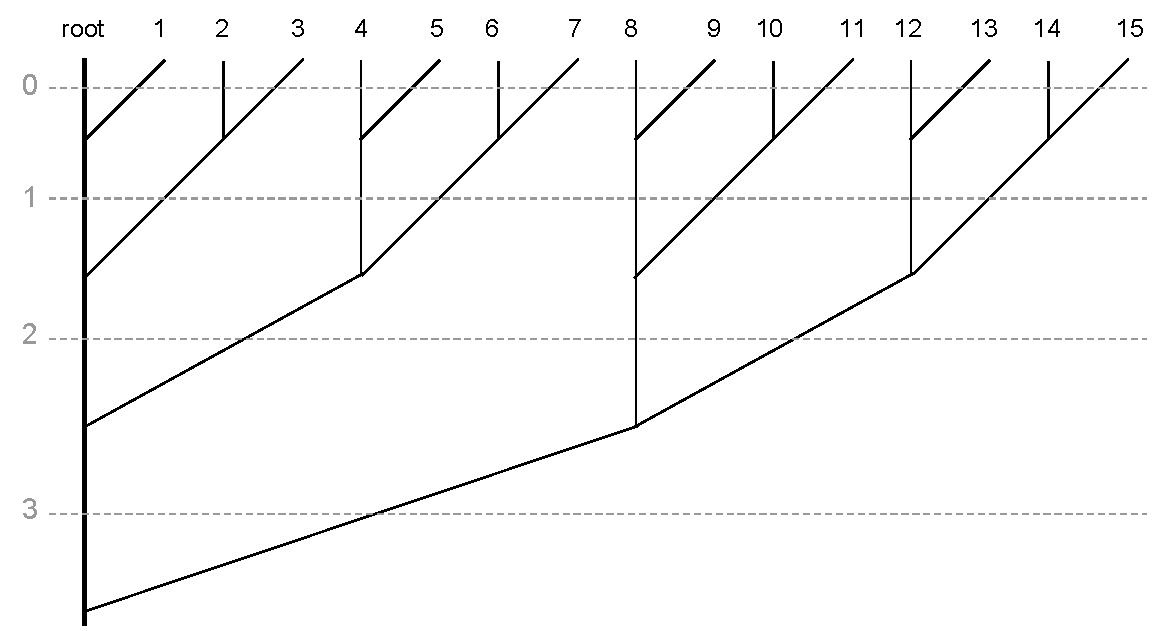
\includegraphics[scale=0.5]{pdf/reduction-tree.pdf}
	\caption[Result reduction calucation example]{Example of a result reduction calucation with 16 storage nodes. \label{fig:reduction-tree}}
\end{figure}	

Each function in the \texttt{OperationContext} is executed in parallel and sequential by the specification from the end-user for the particular procedure. At least one parameter; a block iterator, are required for all functions defined. Hence, the following piece of simple code can be used to iterate over the semantic block content: \texttt{for temp in temperatures: $\ldots$ ;}

\section{Poll}
The poll call is used to check whether the execution of the submitted operation has terminated if the callback of the submit request is vacant.

\section{Documentation}
All the public API calls are documented using Sphinx \cite{PageSphinx} which, using the Python docstring and a \texttt{reStructuredText} markup language layout files is generating intelligent and browsable HTML pages.


\chapter{Nodes} \label{chp:nodes}
\section{General}

\section{Gateway} \label{sec:gateway}

\section{Storage node} \label{sec:storage}
%TODO Menition Real-time scalable access model: NameService due to on the fly calculation of ids on all storage nodes

\section{Monitor} \label{sec:monitor}
%TODO Reference to \ref{sec:recovery} from architecture when writing about live software reboot - also reference to the system configuration \ref{sec:configuration}


\part{Extensions} \label{prt:extensions}
\chapter{A Big Data Analysis Engine} \label{chp:bdae}
\BigLetter{T}{he} purpose and ambition are to create a \CodeName extension build up on the core API explained in chapter \ref{chp:api}, to demonstrate the opportunities with a present example to set a standard. The extension seeks to model a data access layer (DAL) as a MapReduce framework (Definition \ref{def:mapreduce}) for \CodeName like Hadoop for HDFS.

\section{Investigation}
The initial idea were to create a bridge between the DAL of Disco (Section \ref{sec:related}) and the API of \CodeName and thereby create a combined integration of the two systems, so that \CodeName would be an optimized and semantic-intelligent replacement for DDFS (Disco Distributed File System). The Disco end-user experience is written in Python programming language like \CodeName and thus would be more convenient to incorporate, rather than frameworks such as Hadoop, which is written in Java.
\newline

The reason to design and implement an entirely new framework and thereby discard the Disco based solution was due to the demand and desire to have full control across the whole execution stack from the disk to the end-user input fields. A second significant reason is the optimization opportunities of having control of the full implementation such as caching of temporary and final results and data accessing.

\section{Assumption}
A small but sufficient number of assumptions has been put together, based on the brief but necessary investigation and the knowledge obtained by the examination of related work (Section \ref{sec:related}), to limit the extension to the project scope:

\begin{itemize}
	\item The solution is targeted and used for big data analysis.	
	\item Data is assumed to be research and scientific related material. 
\end{itemize}
, which generally is inspired and based on the ones for \CodeName (Section \ref{sec:assumption}).
\newline

Additionally, it is a requirement and thereby an assumption that the \texttt{OperationContext}s (Section \ref{sec:operation}) of the datasets can be modeled in terms of a MapReduce scheme.

\section{Objectives} \label{sec:bdae-objectives}
Based on the assumptions and the general knowledge learned by studying similar frameworks has following objectives been composed:
\begin{itemize}
	\item Utilize the \CodeName storage system and its API to create MapReduce based DAL.
	\item Define and design a collection structure to batch similar datasets.
	\item Implement predefined templates for common data structures to reduce redundant tasks for the end-users.
	\item Characterize a domain specific access model.
	\item Load complex data structures such as NetCDF\cite{PageNetCDF} or HDF5\cite{PageHDF5}\cite{Collette:2013:Python} in an intelligent and thus efficiently way to reduce I/O cost.
\end{itemize}

\section{Overview}
BDAE (\textit{/b'dei'/}) is the name and acronym of the big data analysis engine targeting MapReduce operations that are implemented. The solution is built solely using the \CodeName API as illustrated in Figure \ref{fig:bdae-overview} and extending existing core components primarily from the foundation package.

\begin{figure}
	\centering
	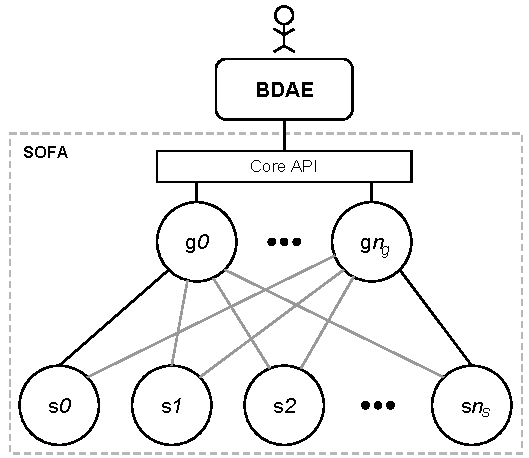
\includegraphics[scale=0.9]{pdf/bdae-overview.pdf}
	\caption[General overview of the BDAE]{General overview of the BDAE integration into \CodeName with same notation as in Figure \ref{fig:sofa-overview}. \label{fig:bdae-overview}}
\end{figure}	


\subsection{Dataset}
The \texttt{SofaBaseObject} (Section \ref{sec:sofabaseobject}) has been extended and delimited along with the requirement of the functions defined in the \texttt{OperationContex}, as a consequence of the chosen execution model. 
\begin{itemize}
	\item A \texttt{MapReduceDataset} has been defined which requires functions executed on the data to be ordered into two categories: \texttt{map} and \texttt{reduce}. 
	\item All functions defined in an extended \texttt{OperationContex} is at runtime verified towards the two categories since the MapReduce execution model prescribes that each operation has at least one map function and at most one reduce function at the end.
\end{itemize}

\section{Collection} \label{sec:collection}
A dataset in \CodeName is defined by a dictionary with metadata and a list of associated semantic blocks, but this metadata structure can with small modifications also be used as a descriptor for a collection of similar datasets, which was one of the objectives (Section \ref{sec:bdae-objectives}):

\begin{quotation}
	\textit{"Define and design a collection structure to batch similar datasets."}
\end{quotation}

In other words; a collection in BDAE is defined as a marginally altered metadata dictionary with zero-length list of associated semantic blocks, that nevertheless obeys the interface of the \texttt{SofaBaseObject}, which is a required for any type of data in \CodeName.

\section{MapReduce}
The tree barrier based operation execution model implemented in \CodeName is well-suited for a MapReduce framework and BDAE is utilizing this straightforward advantage. Figure \ref{fig:reduction-tree} illustrates an example of an execution reduction tree as it would resemble with 16 storage nodes, the figure exemplifies among other things how and when the different storage nodes are communicating to calculate the correct result jointly.
\newline

The joints have an important function in the MapReduce framework and have the overall responsibility of why the execution model adds up and it is implemented as following:
\begin{enumerate}
	\item Each node is executing one or more \texttt{map} functions locally.
	\item The neighbor nodes are based on equation \ref{eq:reduction} calculating the locally combined \texttt{reduce} together.
\end{enumerate}

Figure \ref{fig:map-reduce-tree} illustrates the two steps explained above, where second step is repeated with the same \texttt{reduce} function until all local results are combined to a global result.

\begin{figure}
	\centering
	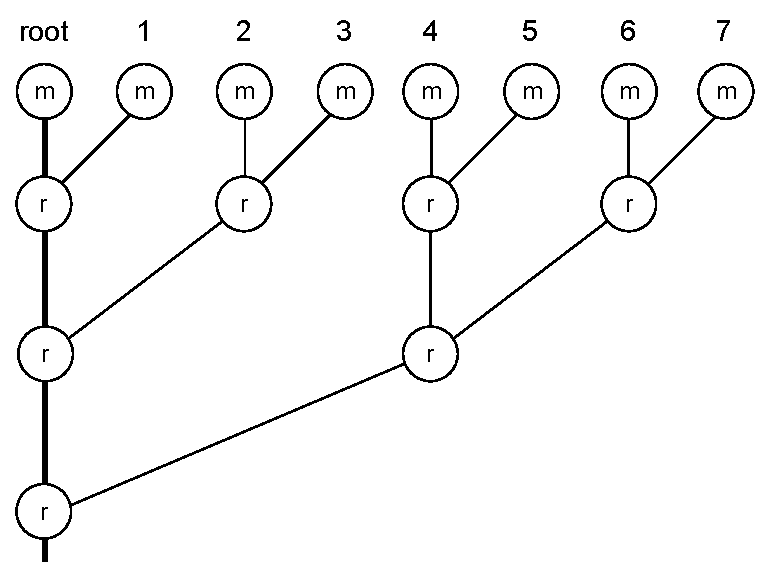
\includegraphics[scale=0.7]{pdf/map-reduce-tree.pdf}
	\caption[BDAE MapReduce implementation]{Utilization of the tree barrier based operation execution model in \CodeName for MapReduce in BDAE. \texttt{m} = map and \texttt{r} = reduce. \label{fig:map-reduce-tree}}
\end{figure}	

\section{User tiers} \label{sec:user-tiers}
One of the objectives for BDAE was to: \textit{"Characterize a domain specific access model"} to first and foremost redeem expectations of system-wide access control, such that the scientist research employees who submit new map reduce operations does not have direct access to boot and teardown servers, as an example.
\newline

The entire BDAE + \CodeName system are divided into three major responsibilities, which each has its domain specific user access level. The responsibilities are inherited as the level increases, which means that the \textbf{data manager} have the same rights as the \textbf{data scientist} and so fourth.
\newline

The core API of \CodeName has been wrapped into a BDAE specific controller that grants access based on user level, in order to restrict the API access and thus accomplish this.

\subsection{Level 1: Data scientist}
Access rights:
\begin{itemize}
	\item Submit new MapReduce operation
	\item Poll for result
	\item Various \texttt{get}-functions to retrieve metadata information regarding the datasets.
\end{itemize}

\subsection{Level 2: Data manager}
Access rights:
\begin{itemize}
	\item Create dataset
	\item Create collection (essentially a thin wrapper around the create dataset API-call with some extra collection specific logic.)
	\item Append data to dataset
	\item Update/delete dataset
\end{itemize}

\subsection{Level 3: System administrator}
Access rights:
\begin{itemize}
	\item Boot and teardown servers
\end{itemize}

\section{Templates} \label{sec:templates}
BDAE provides a range of different abstract templates related to commonly used data types within the field of interest, to reduce excessive workload for the end-users and generalize the final implementation solution, such that solutions to similar problems are easily comparable.
\newline

\noindent
The templates provided includes:
\begin{itemize}
	\item One for \textbf{text} data that can split raw data into semantic blocks by three different properties: \textit{line}, \textit{sentence} or \textit{word}.
	\item A template for \textbf{image} data that simplifies the burden of transforming raw data such as tiff-files into Numpy arrays.
	\item The template for \textbf{Numpy/Bohrium array}'s is a simple solution that uses the template module binder described subsequently to bind regularly used functions from the respective libraries.
	\item One of the objectives listed in Section \ref{sec:bdae-objectives} includes: \textit{"Load complex data structures such as NetCDF $\ldots$ in an intelligent and thus efficiently way to reduce I/O cost."}, which is accomplished by utilizing the collection module (Section \ref{sec:collection}) to create a \textbf{NetCDF} template. This is possible since this data format essentially is a group of related data records. 
\end{itemize}

\subsection{Module binder}
The module binder is not as such a template, but provides opportunities for conveniently binding Python built-in and other third party library functions like \texttt{map} and \texttt{reduce} specific \texttt{OperationContext} functions.
\newline

An example: \texttt{count(}x, y\texttt{)} is a built-in function from the \texttt{string} module in Python \cite{PagePython} that counts number of \texttt{y} in \texttt{x}. The following snippet transforms the \texttt{count(}x, y\texttt{)} into \texttt{count\_occurrences(}x, y\texttt{)} with identical logic parameters and results.
\vspace*{2mm}
\begin{lstlisting}[language=Python, basicstyle=\footnotesize, numbers=none, showtabs=false, showstringspaces=false, showspaces=false, otherkeywords={string,new_fun_names}, stringstyle=\color{blue}]
   module_binder(string, function_binder, ['count'], 
                 new_fun_names=['count_occurrences'])
\end{lstlisting}
\vspace*{-6mm}

\section{Libraries} \label{sec:libraries}
BDAE provides three python libraries one for each of the user tiers (Section \ref{sec:user-tiers}): \texttt{libbdaescientist}, \texttt{libbdaemanager} and \texttt{libbdaeadmin} respectively, that implements the logic listed.

\section{Extensions}
Using the rather simple \CodeName core API it is possible to write useful and comprehensive extensions, as BDAE exemplifies. Likewise it is possible to create extensions on top BDAE using the libraries briefly explained in the previous section. The generic web interface and Android\cite{PageAndroid} application described in this section are two examples of that.

\subsection{Web}
\begin{figure}[h!]
	\centering
	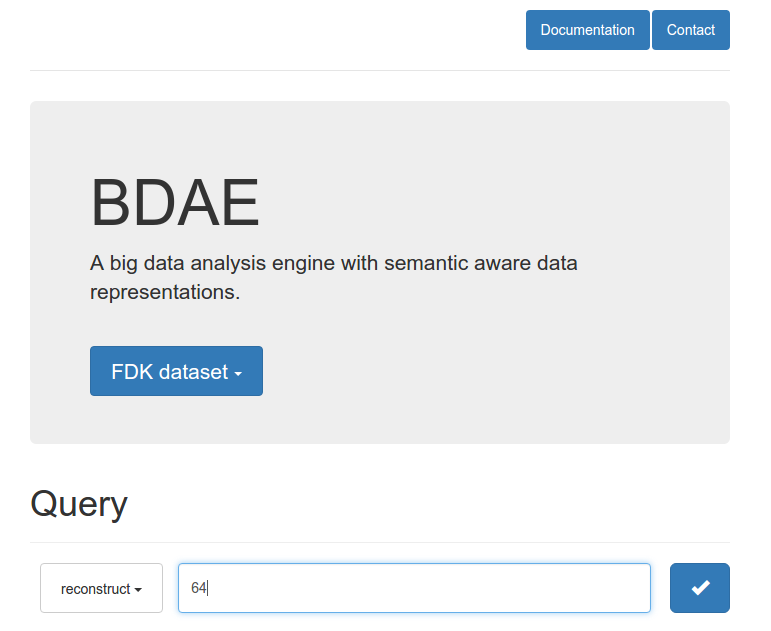
\includegraphics[scale=0.33]{img/website.png}
	\caption{Overview of the BDAE website. \label{fig:website}}
\end{figure}

A simple graphical user interface represented as a website (illustrated in Figure \ref{fig:website}) is provided as part of the BDAE framework installation (explained in Appendix \ref{app:installation}). 
\clearpage

The website expands the options regarding the scientist position, since it is no longer a requirement to master the skill of programming in order to operate BDAE at that user tier. At the moment it is possible to:
\begin{itemize}
	\item Choose the dataset to operate on among all available in \CodeName.
	\item Submit a new MapReduce operation.
	\item And view the result whenever it has finished the execution.
\end{itemize}
, but supporting more features are in the project pipeline.

\subsection{Android application} \label{sec:bdaeapp}
The Android application provides a handheld modern access to the scientist level of BDAE, implemented in a minimalist Google approved material design \cite{PageMaterialDesign} (Figure \ref{fig:app-overview}) (Appendix \ref{chp:app-screenshots}).
\newline

\begin{figure}[h!]
	\centering
	\vspace*{4mm}
	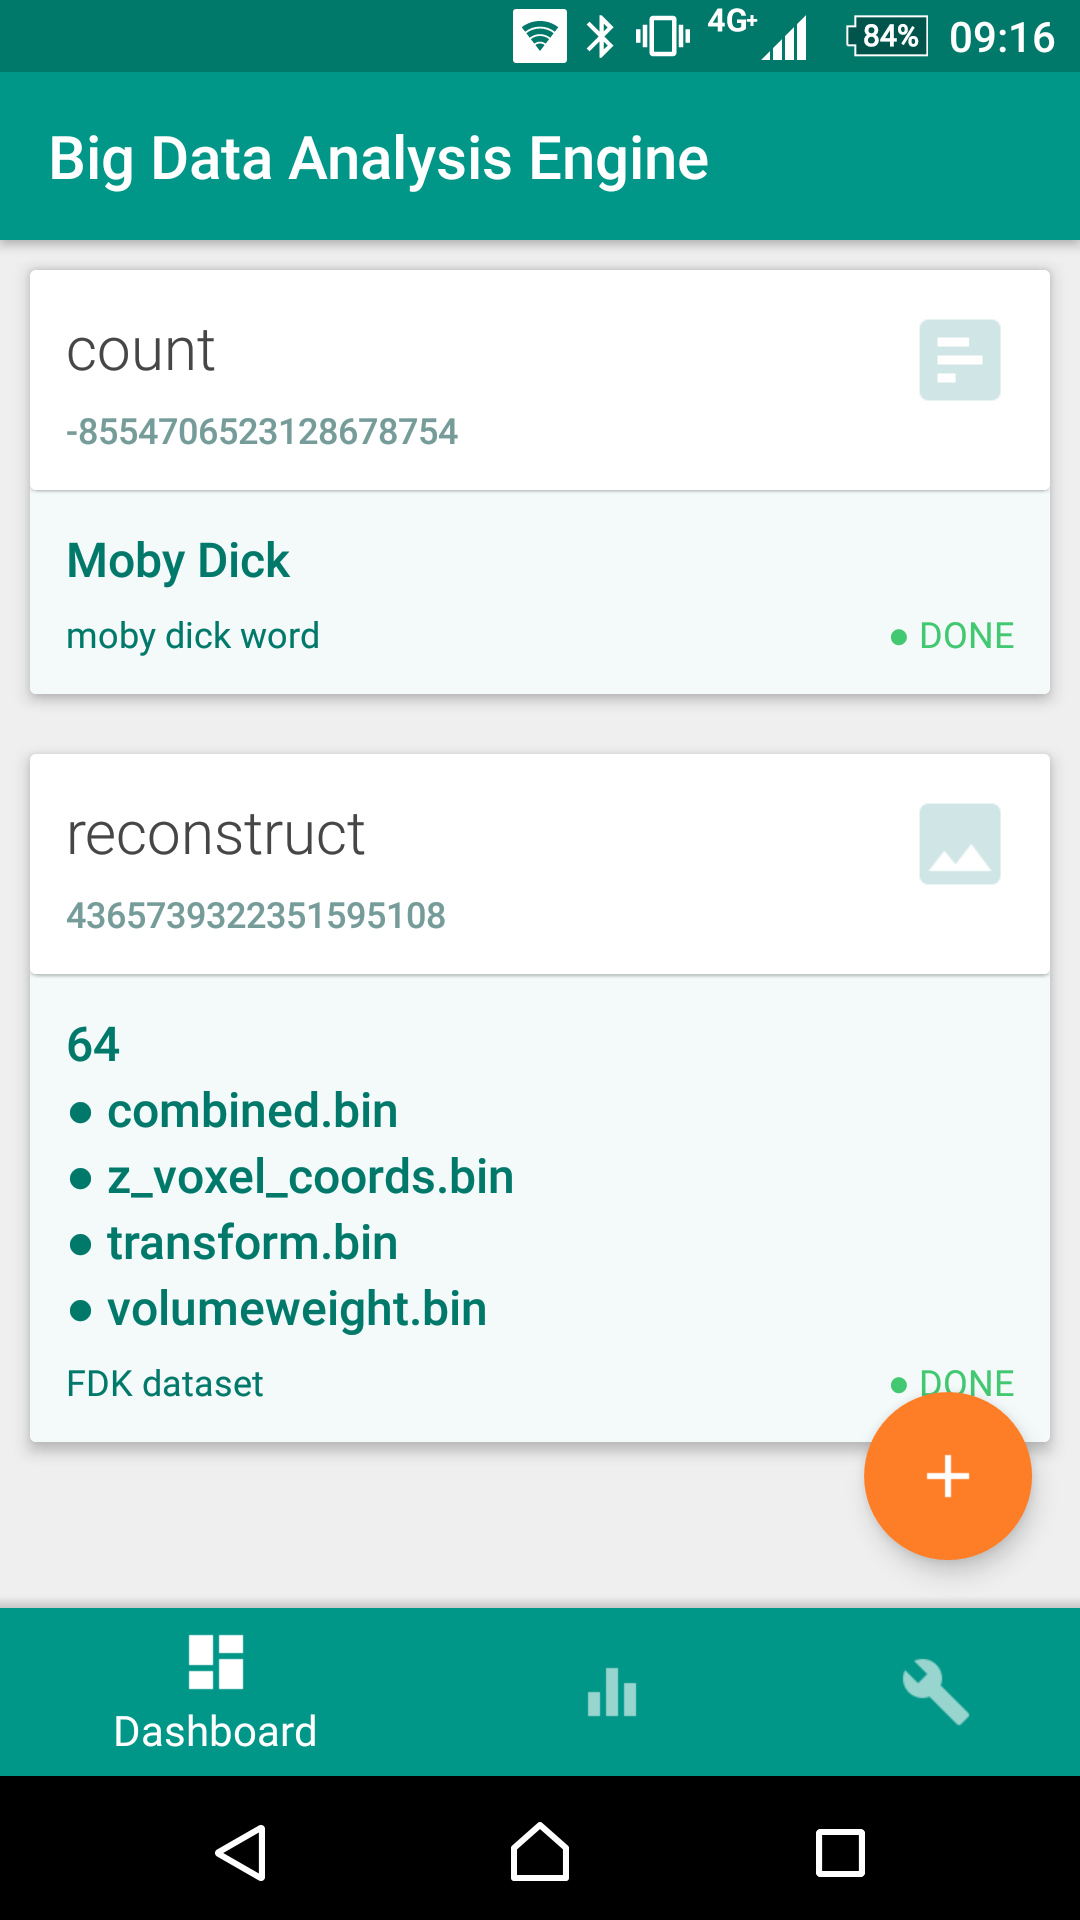
\includegraphics[width=0.4\textwidth]{img/overview.png}
	\caption[Android application overview]{Android application overview of the current MapReduce operations executing in BDAE. \label{fig:app-overview}}
	\vspace*{4mm}
\end{figure}

\noindent
The application supports following features:
\begin{itemize}
	\item Configuration of gateway access server.
	\item All types \CodeName specific instances defined by the \texttt{instance-name} system configuration.
	\item Visualization of current executing MapReduce operations.
	\item Adding new operations for existing datasets.
	\item Listing metadata information about all datasets currently available in \CodeName.
	\item View the results of all the previous executed operations.
\end{itemize}

\section{Example}
The productivity, readability and maintainability levels of \CodeName and BDAE are demonstrated and compared to Hadoop since the implemented prototype is a more or less complete framework. Hadoop was chosen based on the popularity and thus comprehensive usage and thereby plenty of very well-produced examples.
\newline

The example used to illustrate the mentioned features of \CodeName and BDAE is a simple processes of log files to summarize the events by type\cite{PageTomWheeler}. This: \texttt{2013-06-29 22:17:05.362 CDT ERROR "Out of memory"} is an example of a log output and thereby a job input for the \texttt{MapReduce} operation. 
\newline

The map and reduce functions are mainly\footnote{Other languages such as Python are available through the Hadoop Streaming API.} written in Java and thus forces an object-oriented class structure of the function logic. The \texttt{Mapper} and \texttt{Reducer} class representations requires specific and hard coded object types of the input and output parameters, partially due to the programming language restrictions but also because that Hadoop sorts the output of the map function before applying the reduce function.

\subsection{Map}
The map function in BDAE implementing the logic described is defined by a simple 5 line code snippet (Code \ref{lst:bdae-map}), whereas the corresponding Hadoop code is specified by 39 lines of code (Appendix \ref{sec:hadoop-map}).

\begin{lstlisting}[float, basicstyle=\fontsize{8}{5}\selectfont\ttfamily, language=Python, xleftmargin=.8cm, caption={BDAE map function}, label={lst:bdae-map}]
def log_mapper(blocks, levels):
    res = zeros((1, len(levels)))
    for entry in sum(blocks, []):
        res += array([entry.count(level) for level in levels])
    return res
\end{lstlisting}

\subsection{Reduce}
The BDAE reduce function is a simple function with 2 lines of code (Code \ref{lst:bdae-reduce}) that calculates the aggregated amount of log events. The corresponding Hadoop code is 25 lines of code (Appendix \ref{sec:hadoop-reduce}).
\vspace*{4mm}

\begin{lstlisting}[basicstyle=\fontsize{8}{5}\selectfont\ttfamily, language=Python, xleftmargin=0.8cm, caption={BDAE reduce function}, label={lst:bdae-reduce}]
def log_reducer(blocks):
    return array(blocks).sum(axis=0)
\end{lstlisting}

\part{Evaluation} \label{prt:evaluation}
\chapter{Test} \label{chp:test}
A variety of different examples of how to utilize and program BDAE efficiently are provided as part of the installation of the complete framework (a guide is available in appendix \ref{app:installation}), which has been tested and verified throughout the development process. 

Furthermore, a range of the most relevant scenarios are additionally tested and validated with the unit test framework\cite{PageUnitTest} in Python. The following chapter is dedicated to describing the unit tests.

\section{SOFA}
\CodeName was carefully tested as part of the BDAE unit tests, but not as a standalone framework, since it is hard to test alone as it is intended to be a subset of a larger system built on top using the available API. 

The tests of BDAE are utilizing a majority of the available crucial API call\footnote{Not the straightforward \texttt{get} method calls.} of \CodeName and are considered comprehensive enough for now, as BDAE would not functioning correctly or at all if \CodeName did not operate correctly.

\section{BDAE}
The unit test cases are implemented using and thus testing the provided BDAE templates described in section \ref{sec:templates} using the adequate user level based BDAE libraries described in section \ref{sec:libraries}.
\newline

\CodeName + BDAE are additionally tested as part of the performance benchmarking described in chapter \ref{chp:benchmark}.

\subsection*{Text}
The test cases for the text-based data covers all three types of BDAE templates explained in section \ref{sec:templates} and the purpose is it test tangible examples.

\testcase{Letter count}{Counting the total number of letters in an arbitrary generated scientific dataset string}{This test are verified using all the three types of text-based templates: \textit{line}, \textit{sentence} or \textit{word}.}{
	\begin{itemize}
		\item \textbf{M}: Repeat count
		\item \textbf{L}: The letter to be repeated $M$ times, an example for $N=4$ and $L=$'a' results in: a aa aaa aaaa.
		\item \textbf{N}: Replication count
	\end{itemize}
}{
\begin{equation*}
	N \cdot \sum_{m=1}^{M+1} m
\end{equation*}
}{All results are tested with $L$ = 'a'.}{
\centering
\begin{tabular}{l p{3cm}}
\specialrule{1.5pt}{2pt}{2pt}
\textbf{Input} & \textbf{Output} \\
\midrule
$N = 1$, $M=1$ & 1 \\ 
$N = 10$, $M=1$ & 55 \\ 
$N = 10$, $M=10$ & 550 \\ 
\specialrule{1.5pt}{2pt}{2pt}
\end{tabular}
}

\testcase{Line count}{Counting the number lines in an arbitrary generated scientific dataset string}{This test are verified using text-based templates: \textit{line}.}{
	\begin{quotation}
		Same as above.
	\end{quotation}
}{
\begin{equation*}
	M
\end{equation*}
}{All results are tested with $L$ = 'a'.}{
\centering
\begin{tabular}{l p{3cm}}
\specialrule{1.5pt}{2pt}{2pt}
\textbf{Input} & \textbf{Output} \\
\midrule
$N = 1$, $M=1$ & 1 \\ 
$N = 10$, $M=1$ & 1 \\ 
$N = 10$, $M=10$ & 10 \\ 
\specialrule{1.5pt}{2pt}{2pt}
\end{tabular}
}

\testcase{Word count}{Counting the number word (defined as text separated by a space in this situation) in an arbitrary generated scientific dataset string}{This test are verified using text-based templates: \textit{word}.}{
	\begin{quotation}
		Same as above.
	\end{quotation}
	\newpage
}{
\begin{equation*}
	N*M
\end{equation*}
}{All results are tested with $L$ = 'a'.}{
\centering
\begin{tabular}{l p{3cm}}
\specialrule{1.5pt}{2pt}{2pt}
\textbf{Input} & \textbf{Output} \\
\midrule
$N = 1$, $M=1$ & 1 \\ 
$N = 10$, $M=1$ & 10 \\ 
$N = 10$, $M=10$ & 100 \\ 
\specialrule{1.5pt}{2pt}{2pt}
\end{tabular}
}
\vspace*{5mm}

\subsection*{Numpy/Bohrium array}
The test cases for the Numpy/Bohrium array template predominantly focuses on the ability to divide the data correctly into the specified semantic blocks and nevertheless calculate the correct results in multiple and various dimensions.

\testcase{Global sum}{Calculating the global sum of the arbitrary generated scientific single and or multidimensional array of fixed data.}{Tested using full arrays of ones, twos etc.}{
	\begin{itemize}
		\item \textbf{M}: Repeat count
		\item \textbf{n}: The number to be repeated in an $M\cdot M$ array.
		\item \textbf{N}: Replication count
	\end{itemize}
}{
\begin{equation*}
	n \cdot M^2 \cdot N
\end{equation*}
}{}{
\centering
\begin{tabular}{l p{3cm}}
\specialrule{1.5pt}{2pt}{2pt}
\textbf{Input} & \textbf{Output} \\
\midrule
$n = 1$, $M=1$, $N=1$ & 1 \\ 
$n = 1$, $M=100$, $N=1$ & 10000 \\ 
$n = 2$, $M=10$, $N=10$ & 2000 \\ 
\specialrule{1.5pt}{2pt}{2pt}
\end{tabular}
}

\testcase{Semantic sum}{Calculating the semantic block sum (assumed to be of dimension $(1 \cdot M)$) of the arbitrary generated scientific single and or multidimensional array of fixed data and verifying that all element results are equal.}{The result is either the sum or -1 if the results are not equal.}{
	\begin{quotation}
		Same as above.
	\end{quotation}
}{
\begin{equation*}
	n \cdot M (\cdot 1)
\end{equation*}
}{Assuming $N=1$ as it is independent and thus does not effect the results.}{
\centering
\begin{tabular}{l p{3cm}}
\specialrule{1.5pt}{2pt}{2pt}
\textbf{Input} & \textbf{Output} \\
\midrule
$n = 1$, $M=1$ & 1 \\ 
$n = 1$, $M=100$ & 100 \\ 
$n = 2$, $M=10$ & 20 \\ 
\specialrule{1.5pt}{2pt}{2pt}
\end{tabular}
}
\newpage

\subsection*{NetCDF}

\chapter{Benchmark} \label{chp:benchmark}
\BigLetter{T}{he} benchmarks for the combined BDAE and \CodeName framework will primarily focus on two real world data and computationally heavy applications in big data analysis and image processing namely; Computed Tomographic (CT) reconstruction and Circle detection.
\newline

The benchmarks are executed on an Ubuntu 14.04 LTS (Trusty Tahr)\cite{PageUbuntu1404} cluster with 8 nodes each with following specifications:
\vspace*{5mm}
\begin{table}[h!]
	\centering
	\begin{tabular}{l l}
		\textbf{CPU} & AMD Opteron 6272 \emph{Interlagos} \\
		\textbf{Processor frequency (GHz)} & 2.1 \\
		\textbf{\# cores} & 32 (dual socket) \\
		\textbf{Memory (GB)} & 128 \\
		\textbf{SSD Storage (GB)} & 128 
	\end{tabular}
	\caption{Environment specifications.\label{tab:specifications}}
\end{table}

\section{CT reconstruction}
In the healthcare industry tomographic imaging is widely used for confirming injuries such as broken bones. The reconstruction (Figure \ref{fig:ct}) can be simulated by a mathematical model for transforming a series of at least 180 degrees\footnote{The rest of the 180 degrees is simply a mirror of the others.} of 2D images (\textit{projections}) into a 3D volume (\textit{reconstruction}).
\newpage

\begin{figure}
	\vspace*{3mm}
	\centering
	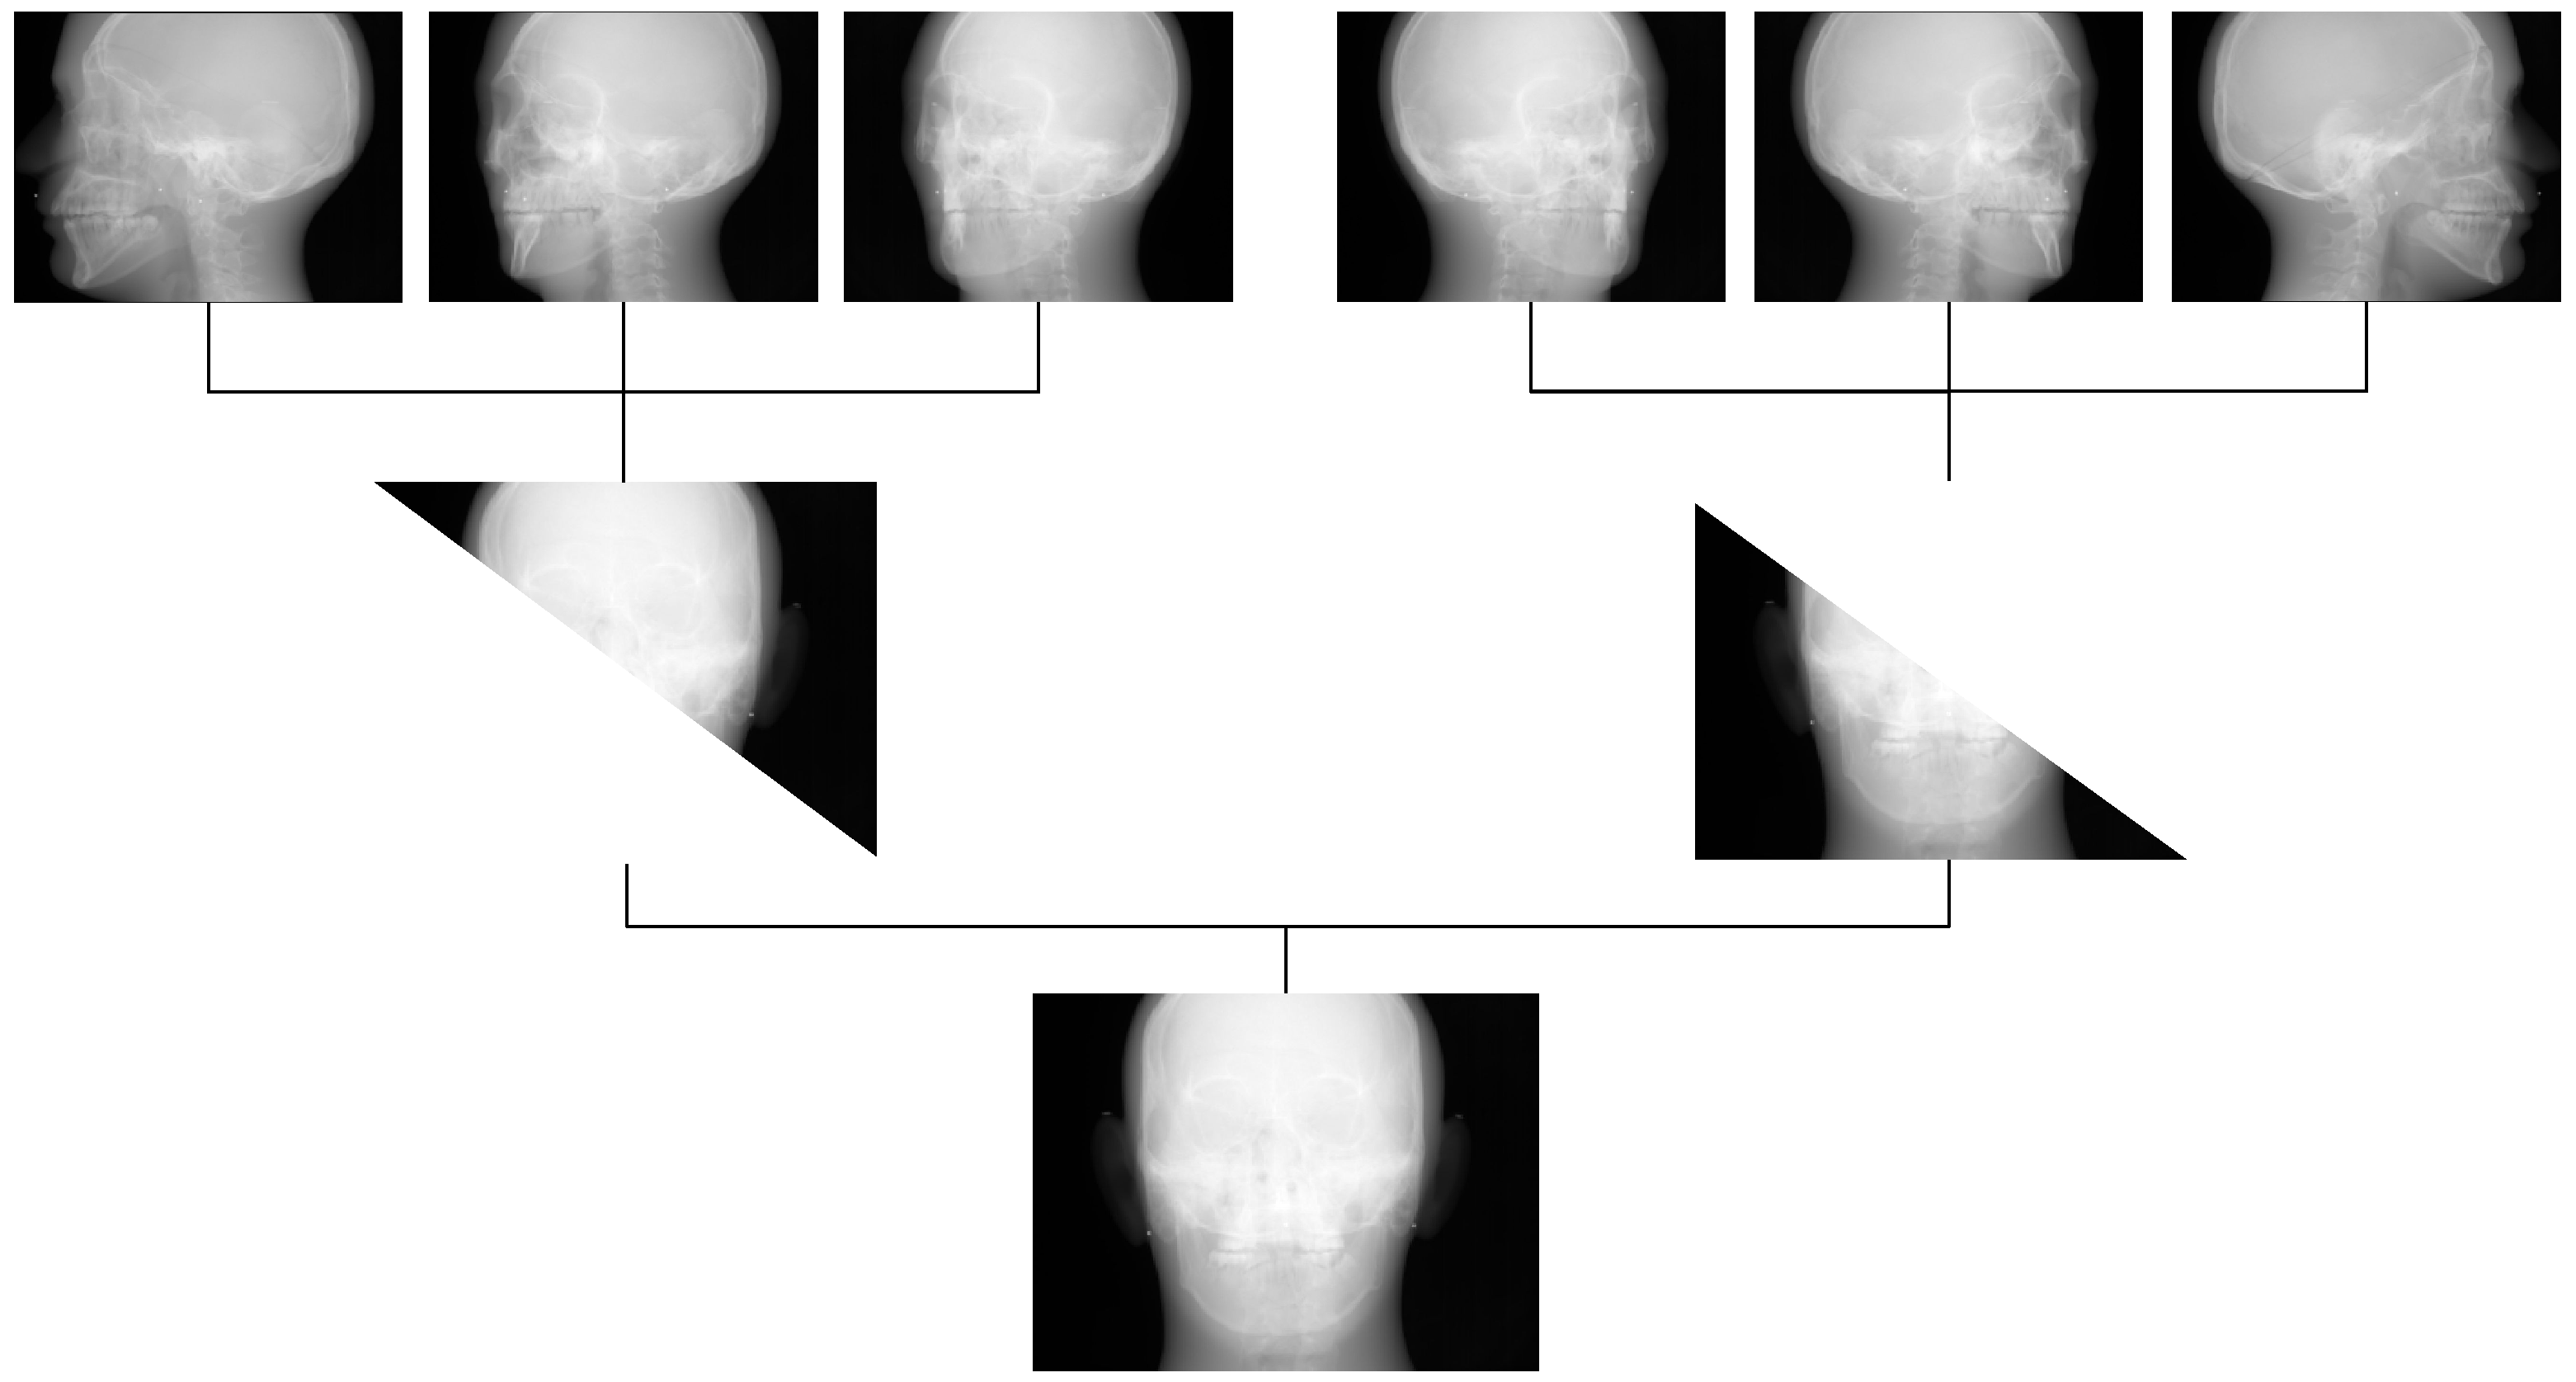
\includegraphics[scale=0.25]{pdf/CT.pdf}
	\caption[]{An example of a distributed parallel CT reconstruction where the second (middle) step is a simulated result to illustrate the notion of a partial volume. \label{fig:ct}}
	\vspace*{3mm}
\end{figure}

\noindent
Simulation results are computed by the cone-beam step-and-shoot method based on the inverse Radon transform known as the filtered back projection algorithm which requires several steps. This benchmark, however, is a simplified version that concentrates on the primary part of the calculation using following precalculated values and partial results:

\begin{itemize}
	\item Preprocessed 2D projects.
	\item Combination of all \texttt{(x, y)} coordinates for the resulting 3D volume.
	\item \texttt{z} coordinates for the 3D volume.
	\item Mapping between 3D and 2D coordinates.
	\item Compensating weights for the cone-beam effect.
\end{itemize}

\subsection*{Simulation results}
The sequential implementation of the CT reconstruction simulation is used as a baseline for calculating the speedup based on the runtime from executing it using the BDAE and \CodeName framework.
\newpage

The sequential source code is rewritten using the Numpy array template (Section \ref{sec:templates}) based on the BDAE \texttt{MapReduceDataset}. The 2D projections are loaded as part of the preprocessing step (Section \ref{sec:sofabaseobject}) and distributed using the chosen distribution strategy.

\begin{itemize}
	\item The \texttt{map} function is basically the sequential code with a reduced number of iterations\footnote{Based on the distribution strategy and the number of storage nodes}.
	\item The \texttt{reduce} function reduces the partial results by applying a universal add operation recursively along the required axis.
\end{itemize}

The CT reconstruction code is executed on three different datasets in increasing volume, and the expectations for the results are that the performance of BDAE will rise the larger the data. Figure \ref{fig:fdk-speedup} presents the speedup results of BDAE compared to the sequential implementation of the CT reconstruction (Graphs of the execution times are in Appendix \ref{app:fdk}).

\begin{figure}[h!]
	\centering
	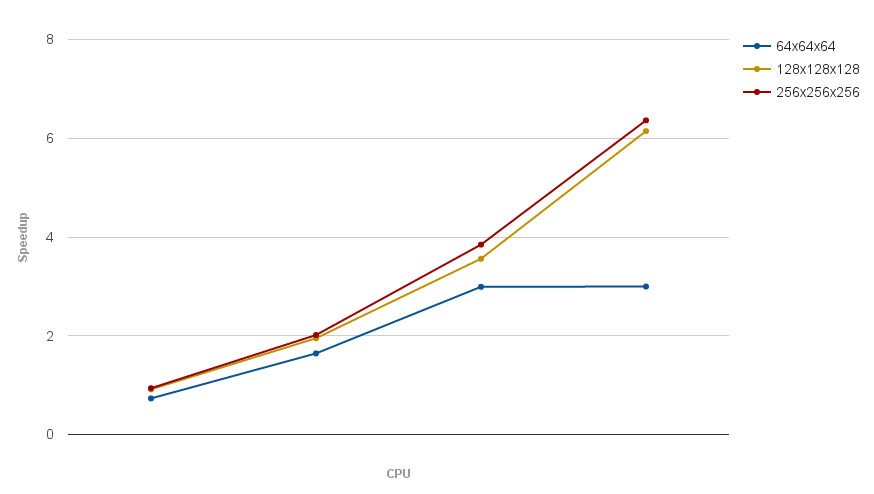
\includegraphics[scale=0.4]{img/fdk-speedup.png}
	\caption[]{Speedup gained using BDAE on the three different datasets. \label{fig:fdk-speedup}}
\end{figure}

The speedup gained is constant using four or more storage nodes on the small 64x64x64 voxels dataset as expected, this is due to the network communication overhead which is dominating the combined execution time. Otherwise, the speedup is quite satisfactory considering the fact that the communication protocol is based on the pure Python library Pyro4 (Section \ref{sec:general}) which: \textit{"$\ldots$ is not designed to efficiently transfer large amounts of binary data over the network. Try to find another protocol that better suits this requirement"}\cite{PagePyro4}.

\section{Circle detection}
One of the useful and productive features in BDAE the ability to transform sequential code into a MapReduce operation with minimal programming effort and without profound knowledge of how the code works. All it takes is: 
\begin{itemize}
	\item Identify the reduction part and determine the need for ghosts (Section \ref{sec:operation}) in the original code.
	\item Define the data using on the of available BDAE templates (Section \ref{sec:templates}) or by extending the \texttt{MapReduceDataset} (Section \ref{sec:bdae-overview}).
	\item Combine the specified \texttt{map} and \texttt{reduce} functions in a operation (Section \ref{sec:operation}) to produce the expected result.
\end{itemize}

\vspace*{3mm}
\noindent
The next benchmark: \textit{Circle detection}, has been implemented using this described blackbox strategy with existing physics code divided into following steps:
\begin{itemize}
	\item \texttt{map}: Median filter.
	\item \texttt{map}: Thresholding.
	\item \texttt{neighborhood:2} (Built-in keywords section \ref{sec:operation}).
	\item \texttt{map}: Eroding.
	\item \texttt{map}: Local connected components.
	\item \texttt{reduce}: Find connected groups.
\end{itemize}

\subsection*{Simulation results}



\chapter{Conclusion} \label{chp:conclusion}
\input{tex/conclusion.tex}

\part{Epilogue} \label{prt:epilogue}
\chapter{Future work} \label{chp:future-work}
\section{Optimizing I/O interactions}
Andersen has designed the concept of a Low-Level Object Store (L-LOS) and implemented a prototype in Python\cite{andersen2016} to optimize the \texttt{shelf} module used for emulating disks. The purpose is to provide an efficient low-level support for storing data based on multiple processes and memory mapped file I/O. The L-LOS framework will contribute as a filesystem in userspace (FUSE) separately on each storage node (Figure \ref{fig:sofa-llos-extension}) and operate at a software stack low-level and are responsible for all I/O interactions with the hard drive disks.

\begin{figure}
	\centering
	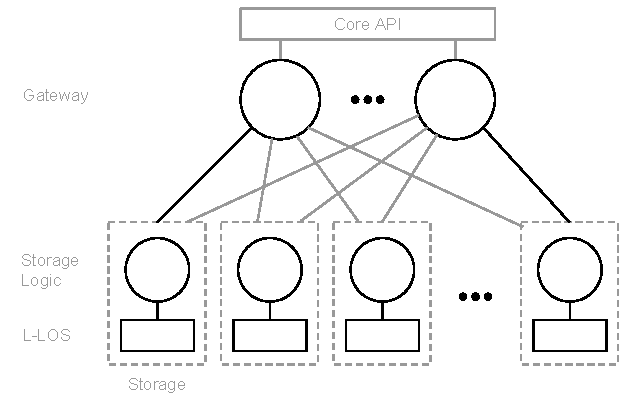
\includegraphics[scale=0.95]{pdf/sofa-llos-extension.pdf}
	\caption{L-LOS integration in \CodeName. \label{fig:sofa-llos-extension}}
\end{figure}

\section{Pipeline support}
A prioritized future implementation is to replace the Python Pyro4 communication library possible with one of the alternatives (Section \ref{sec:communication}) that supports streaming to reduce the package latency, by implement the pipeline solution of the delegation framework (Section \ref{sec:delegation}) and the package distribution protocol in the append API call \ref{sec:api-append}.

\section{Parallel nodes}
As a consequence of the pipeline support and thereby the elimination of the existing communication library it is a demand and crucial for the future work to implement a proper protocol for handling multiple requests in parallel.

\section{Import/export extension}
Use \CodeName as a data transformation framework to unify data formats across multiple different input formats, by creating two new extensions for \CodeName at the same level as BDAE (Figure \ref{fig:bdae-extension}). The ambition is to create two generic self-awareness protocol-based data conversion frameworks where the end-users can specify input data\footnote{By url, path or other common formats.} and a result data format protocol such as HDF5 or NetCDF.

\begin{figure}
	\centering
	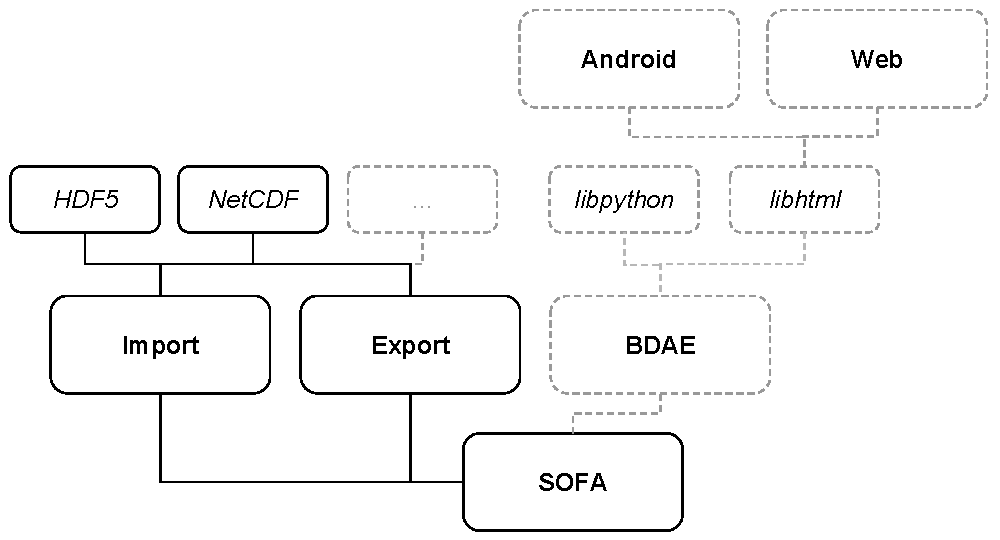
\includegraphics[scale=0.7]{pdf/bdae-extension.pdf}
	\caption{Import/export extension for \CodeName. \label{fig:bdae-extension}}
\end{figure}

\section{Security layer}
Implement an extended access protection layer opportunity at a dataset level by expanding the existing metadata structure with one of following two options:
\begin{enumerate}
	\item A public-key cryptography scheme such that it is only users with matching keys that have access to the data, such scheme is a way to identify trusted entities without involving password and used in protocols such as SSH.
	\item Maintaining a list of verified user identifiers and validate against it before any type operations involving the dataset.
\end{enumerate}

\section{Data encryption}
Implement an encryption/decryption layer which is optional to implement for the end-user and thus can be tailored specifically for individual dataset or applications. Such layer will facilitate options for storing and analyzing personally identifiable data out of the box in \CodeName. 
\newline

A straightforward solution extends the append flow (Figure \ref{fig:preprocess-nextentry}) such that each block is locally encrypted before distributed to the replicas. The decryption, on the other hand, has to be performed at a block level whenever an operation is executed.

\section{Enhanced benchmarks}
A final and evidently relevant task for the future is to implement an extended benchmark suite to compare \CodeName + BDAE against Hadoop and other big data analysis frameworks targeting the same audiences. The extensive comparison between the frameworks is only relevant whenever the rest of the optimizations and prioritized tasks described in this chapter has been applied.


\appendix
\chapter{Installation Guide} \label{app:installation}
\BigLetter{A}{} installation guide\footnote{Linux-based operation system is preferred} for both \CodeName and BDAE including an available test and example suite with samples such as the ones explained in section \ref{sec:examples} in the analysis phase of \CodeName. The source code archive\footnote{\texttt{<project path>/src/}} of the combined project will onwards be referenced as \texttt{src/} and assumed to be fetched from the repository.

\begin{enumerate}
	\item Install \CodeName:
	
	\begin{lstlisting}[numbers=none, backgroundcolor=\color{sourcebackground}, rulecolor=\color{sourcebackground}, framextopmargin=5pt, framexbottommargin=5pt, frame=tb, xrightmargin=15pt]
	cd src/sofa-project
	bash install.sh
	\end{lstlisting}
	\vspace*{-6mm}
	\item Install BDAE:
	
	\begin{lstlisting}[numbers=none, backgroundcolor=\color{sourcebackground}, rulecolor=\color{sourcebackground}, framextopmargin=5pt, framexbottommargin=5pt, frame=tb, xrightmargin=15pt]
	cd src/bdae-project
	bash install.sh
	\end{lstlisting}
	\vspace*{-6mm}
	\item Create new empty project directory\footnote{Will ahead be denoted as \texttt{example/}}.
	\item Duplicate and modify the system configuration file to fit the purpose:
	
	\begin{lstlisting}[numbers=none, backgroundcolor=\color{sourcebackground}, rulecolor=\color{sourcebackground}, framextopmargin=5pt, framexbottommargin=5pt, frame=tb, xrightmargin=15pt]
	cd example
	cp $SOFA_HOME/sofa/sofa.cfg my_sofa.cfg
	vim my_sofa.cfg
	\end{lstlisting}
	
	\item Enable local SSH\footnote{Extra step on macintosh-based systems available here: \url{http://www.techradar.com/how-to/computing/apple/how-to-enable-ssh-on-your-mac-1305644}} to fully utilize the supplied boot-scripts (explained and exemplified in appendix \ref{app:execution}):
	
	\begin{lstlisting}[numbers=none, backgroundcolor=\color{sourcebackground}, rulecolor=\color{sourcebackground}, framextopmargin=5pt, framexbottommargin=5pt, frame=tb, xrightmargin=15pt, commentstyle=\color{bashcommetcolor}]
	cd ~/.ssh/
	touch authorized_keys
	cat id_rsa.pub > authorized_keys
	
	# Verify by ssh to localhost
	ssh localhost
	\end{lstlisting}
	\vspace*{-6mm}
	\item Install following extra Python 2.7 packages to run all BDAE examples, located in \texttt{\$BDAE\_HOME/examples}:

	\begin{lstlisting}[numbers=none, backgroundcolor=\color{sourcebackground}, rulecolor=\color{sourcebackground}, framextopmargin=5pt, framexbottommargin=5pt, frame=tb, xrightmargin=15pt, commentstyle=\color{bashcommetcolor}, showstringspaces=false]
	# Prerequisite for text.py
	pip install ntlk
	python -c "import nltk; nltk.download('punkt')"
	
	# Prerequisite for avs5m.py
	pip install tifffile
		
	# Prerequisite for NetCDF pop.py
	pip install netCDF4
	\end{lstlisting}
	\vspace*{-6mm}
	\item[$\bullet$] {\sffamily\textbf{NOTE:}} To uninstall \CodeName and BDAE, use following two commands:
	\begin{lstlisting}[numbers=none, backgroundcolor=\color{sourcebackground}, rulecolor=\color{sourcebackground}, framextopmargin=5pt, framexbottommargin=5pt, frame=tb, xrightmargin=15pt, commentstyle=\color{bashcommetcolor}, showstringspaces=false]
	cd src/
	bash clean.sh sofa
	bash clean.sh bdae		
	\end{lstlisting}
\end{enumerate}


\chapter{Execution Guide} \label{app:execution}
{\footnotesize \textit{Assuming the installation guide at appendix \ref{app:installation} is completed.}}
\newline

\BigLetter{A}{} general boot script is provided as part of the installation of \CodeName and can succesfully initialize all three type of server. The script requires that the SSH (explained in appendix \ref{app:installation}) is properly configured on each machine.
\begin{itemize}
	\begin{lstlisting}[numbers=none, backgroundcolor=\color{sourcebackground}, rulecolor=\color{sourcebackground}, framextopmargin=5pt, framexbottommargin=5pt, frame=tb, xrightmargin=15pt, commentstyle=\color{bashcommetcolor}, showstringspaces=false, deletendkeywords={file, list}]
	cd $SOFA_HOME/
	
	# General pattern for the boot script
	bash boot.sh <path to cfg file> <state>
	\end{lstlisting}
	\vspace*{-6mm}

	\item Gateway example:
	\begin{lstlisting}[numbers=none, backgroundcolor=\color{sourcebackground}, rulecolor=\color{sourcebackground}, framextopmargin=5pt, framexbottommargin=5pt, frame=tb, xrightmargin=15pt, commentstyle=\color{bashcommetcolor}, showstringspaces=false]
	bash boot.sh example/my_sofa.cfg gateway storage
	\end{lstlisting}
	\vspace*{-6mm}
	
	\item Storage example:
	\begin{lstlisting}[numbers=none, backgroundcolor=\color{sourcebackground}, rulecolor=\color{sourcebackground}, framextopmargin=5pt, framexbottommargin=5pt, frame=tb, xrightmargin=15pt, commentstyle=\color{bashcommetcolor}, showstringspaces=false]
	bash boot.sh example/my_sofa.cfg storage
	\end{lstlisting}
	\vspace*{-6mm}
	
	\item Monitor example:
	\begin{lstlisting}[numbers=none, backgroundcolor=\color{sourcebackground}, rulecolor=\color{sourcebackground}, framextopmargin=5pt, framexbottommargin=5pt, frame=tb, xrightmargin=15pt, commentstyle=\color{bashcommetcolor}, showstringspaces=false]
	bash boot.sh example/my_sofa.cfg monitor storage gateway
	\end{lstlisting}	
\end{itemize}

Note that the \texttt{state} parameter is a list of node types, where the first element is the kind that the current node will adapt. The rest of the optional element in the list is the kind of nodes that the current one will have an awareness of.
\newline

The nodes are bootable by the python daemon too, in the case of misconfigured SSH or other reasons:
\vspace*{2mm}

\begin{lstlisting}[numbers=none, backgroundcolor=\color{sourcebackground}, rulecolor=\color{sourcebackground}, framextopmargin=5pt, framexbottommargin=5pt, frame=tb, xrightmargin=15pt, commentstyle=\color{bashcommetcolor}, showstringspaces=false, deletendkeywords={file, list}]
	python $SOFA_HOME/sofa/boot.py <unique node index> <path to cfg file> <state>
\end{lstlisting}	

{\sffamily\textbf{NOTE:}} A Pyro4 NameService\footnote{Command: \texttt{pyro4-ns}}, one gateway and one storage node is a bare minimum to get started.

\chapter{Application Screenshots} \label{chp:app-screenshots}

\begin{figure*}[h!]
	\centering
  	\begin{minipage}[b]{0.4\textwidth}
    		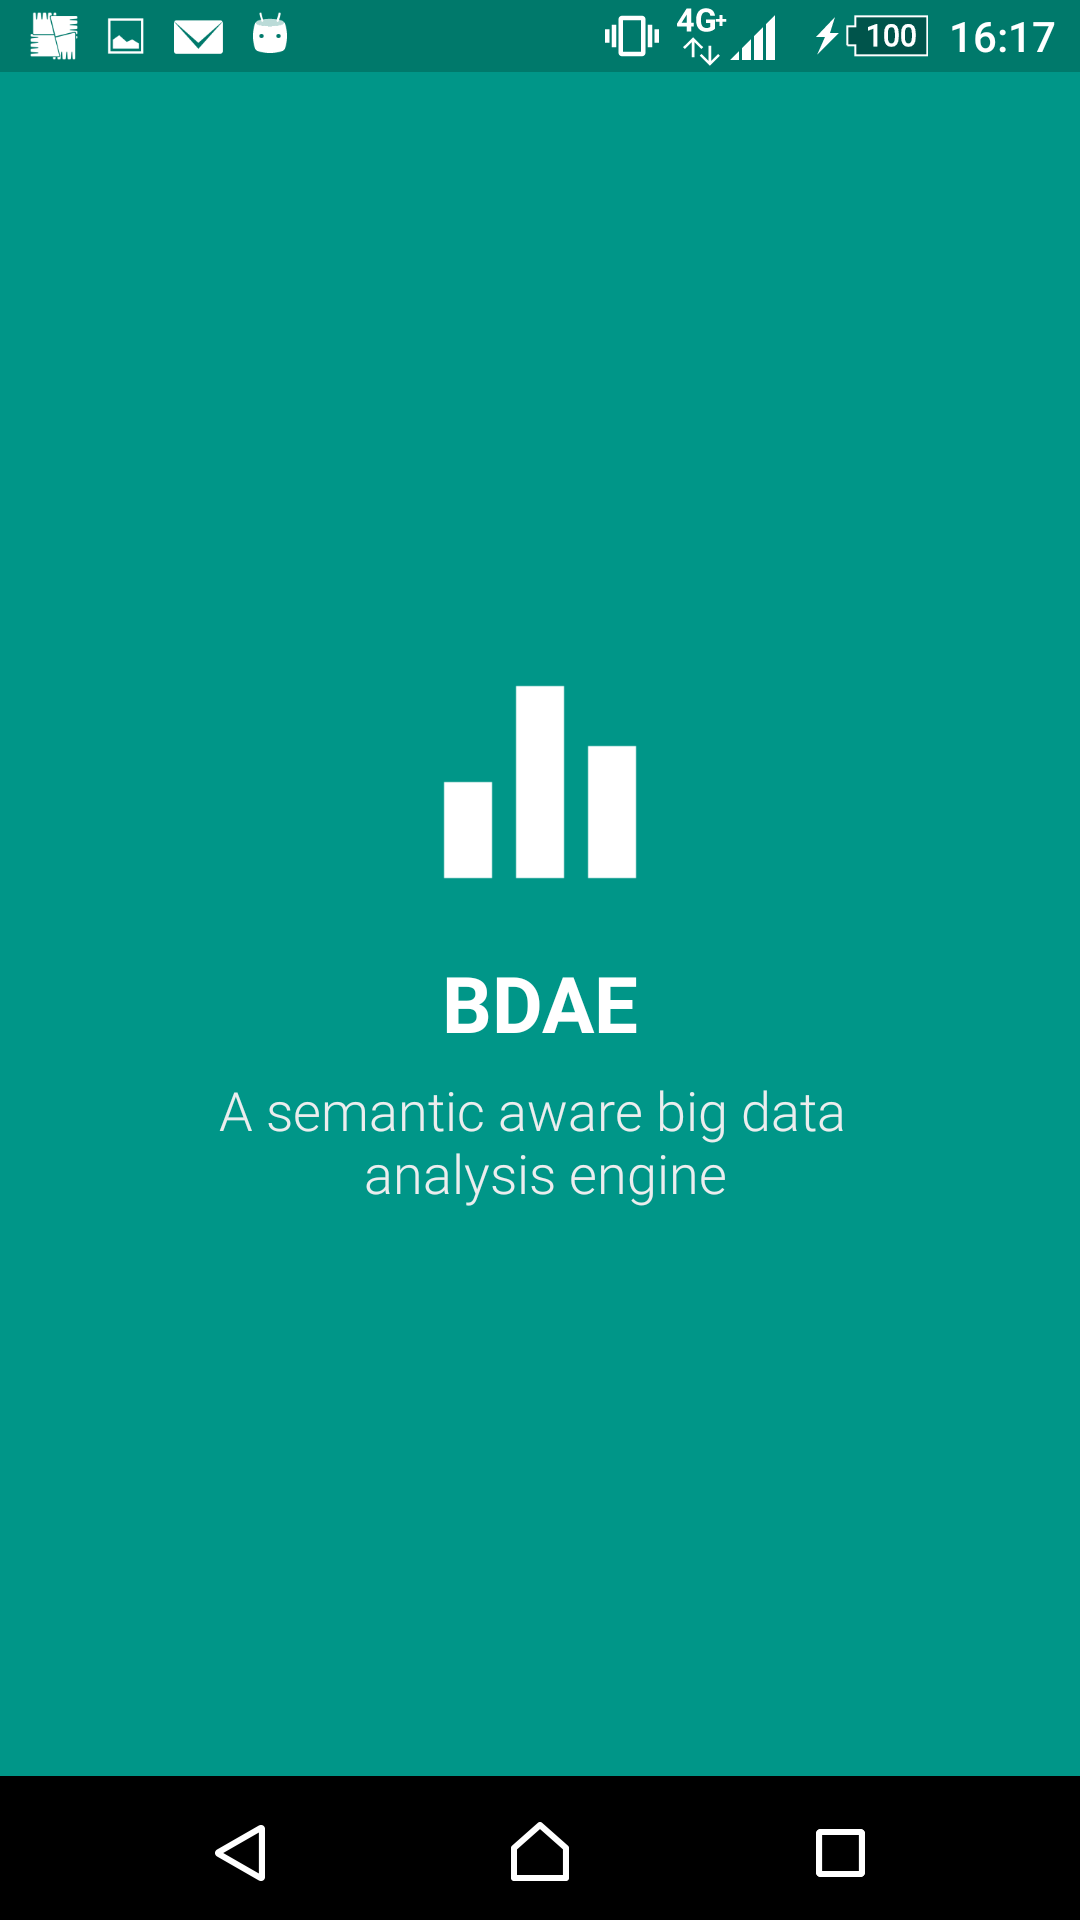
\includegraphics[width=\textwidth]{img/loadingscreen.png}
    \end{minipage}
  	\hfill
  	\begin{minipage}[b]{0.4\textwidth}
    		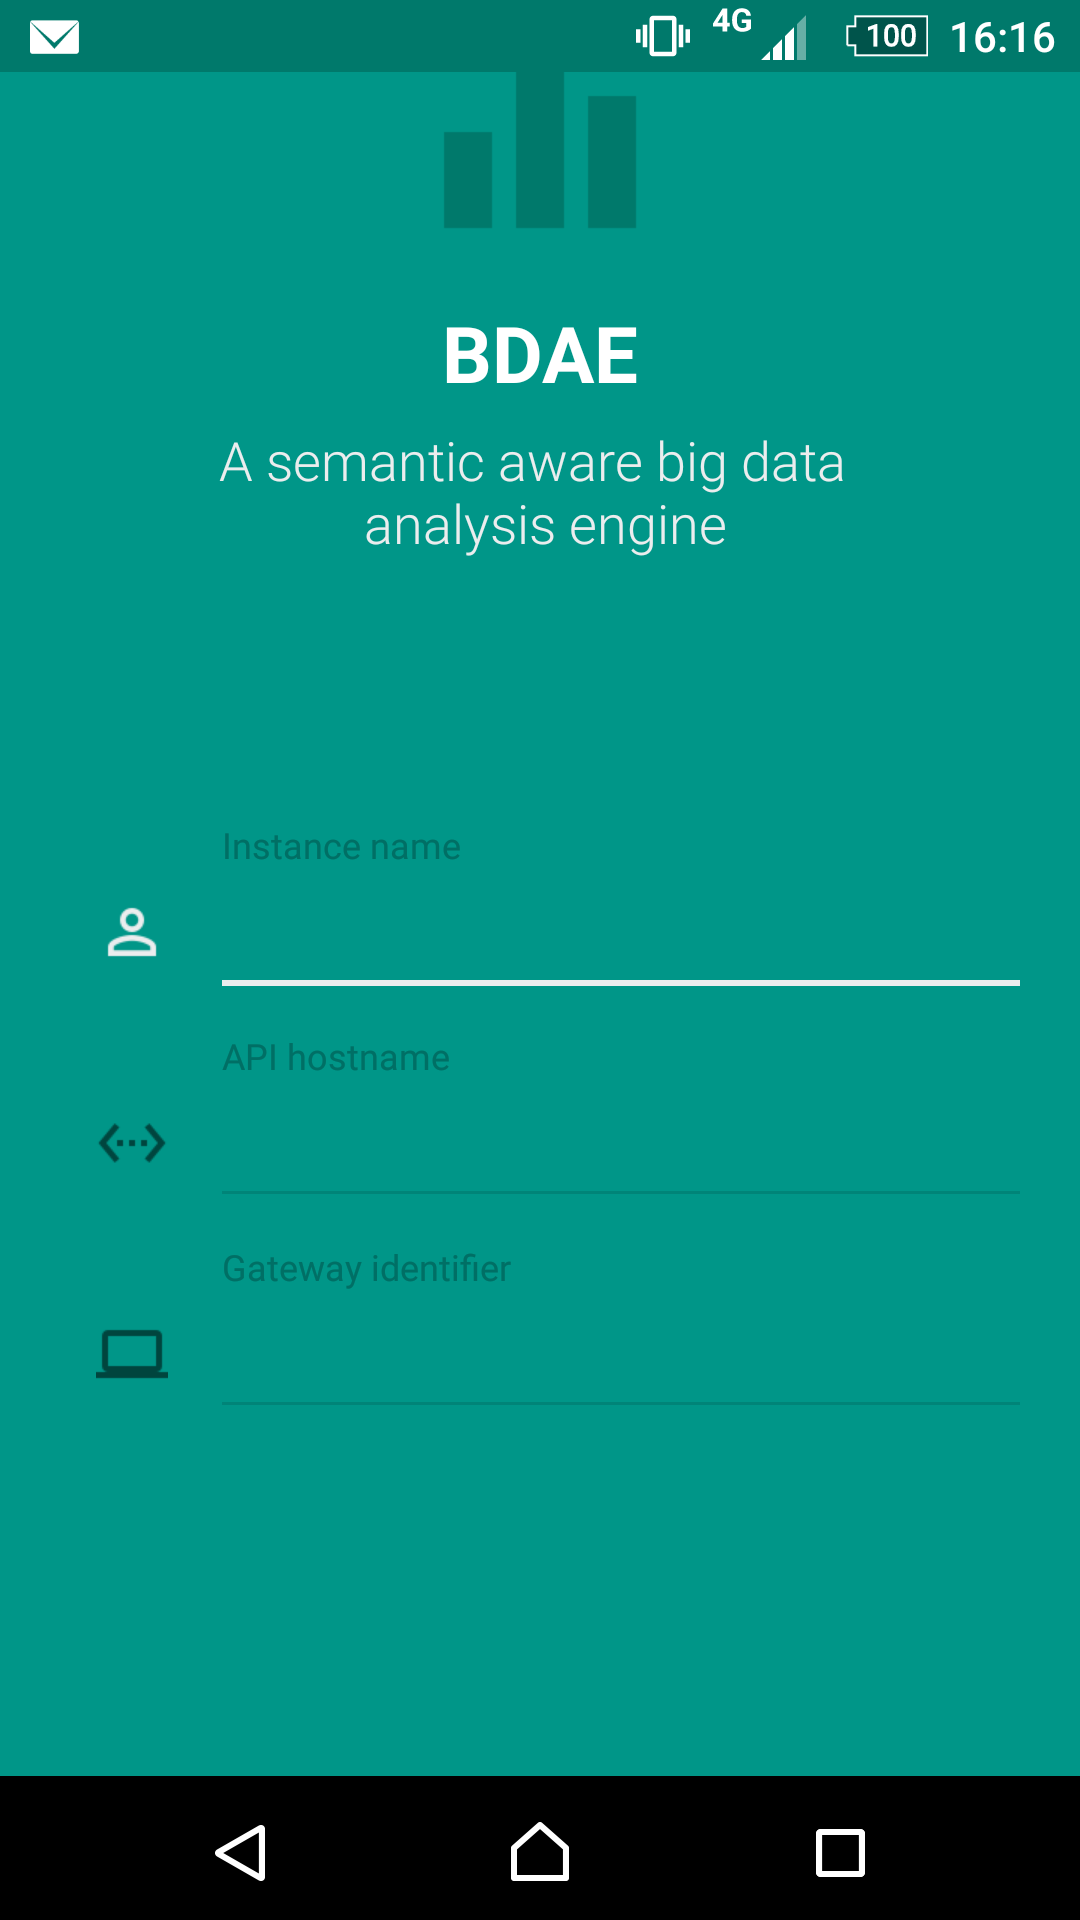
\includegraphics[width=\textwidth]{img/information.png}
  	\end{minipage}
  	\caption[]{Loading screen animated into the required information screen.}
\end{figure*}

\begin{figure*}[h!]
	\centering
  	\begin{minipage}[b]{0.4\textwidth}
    		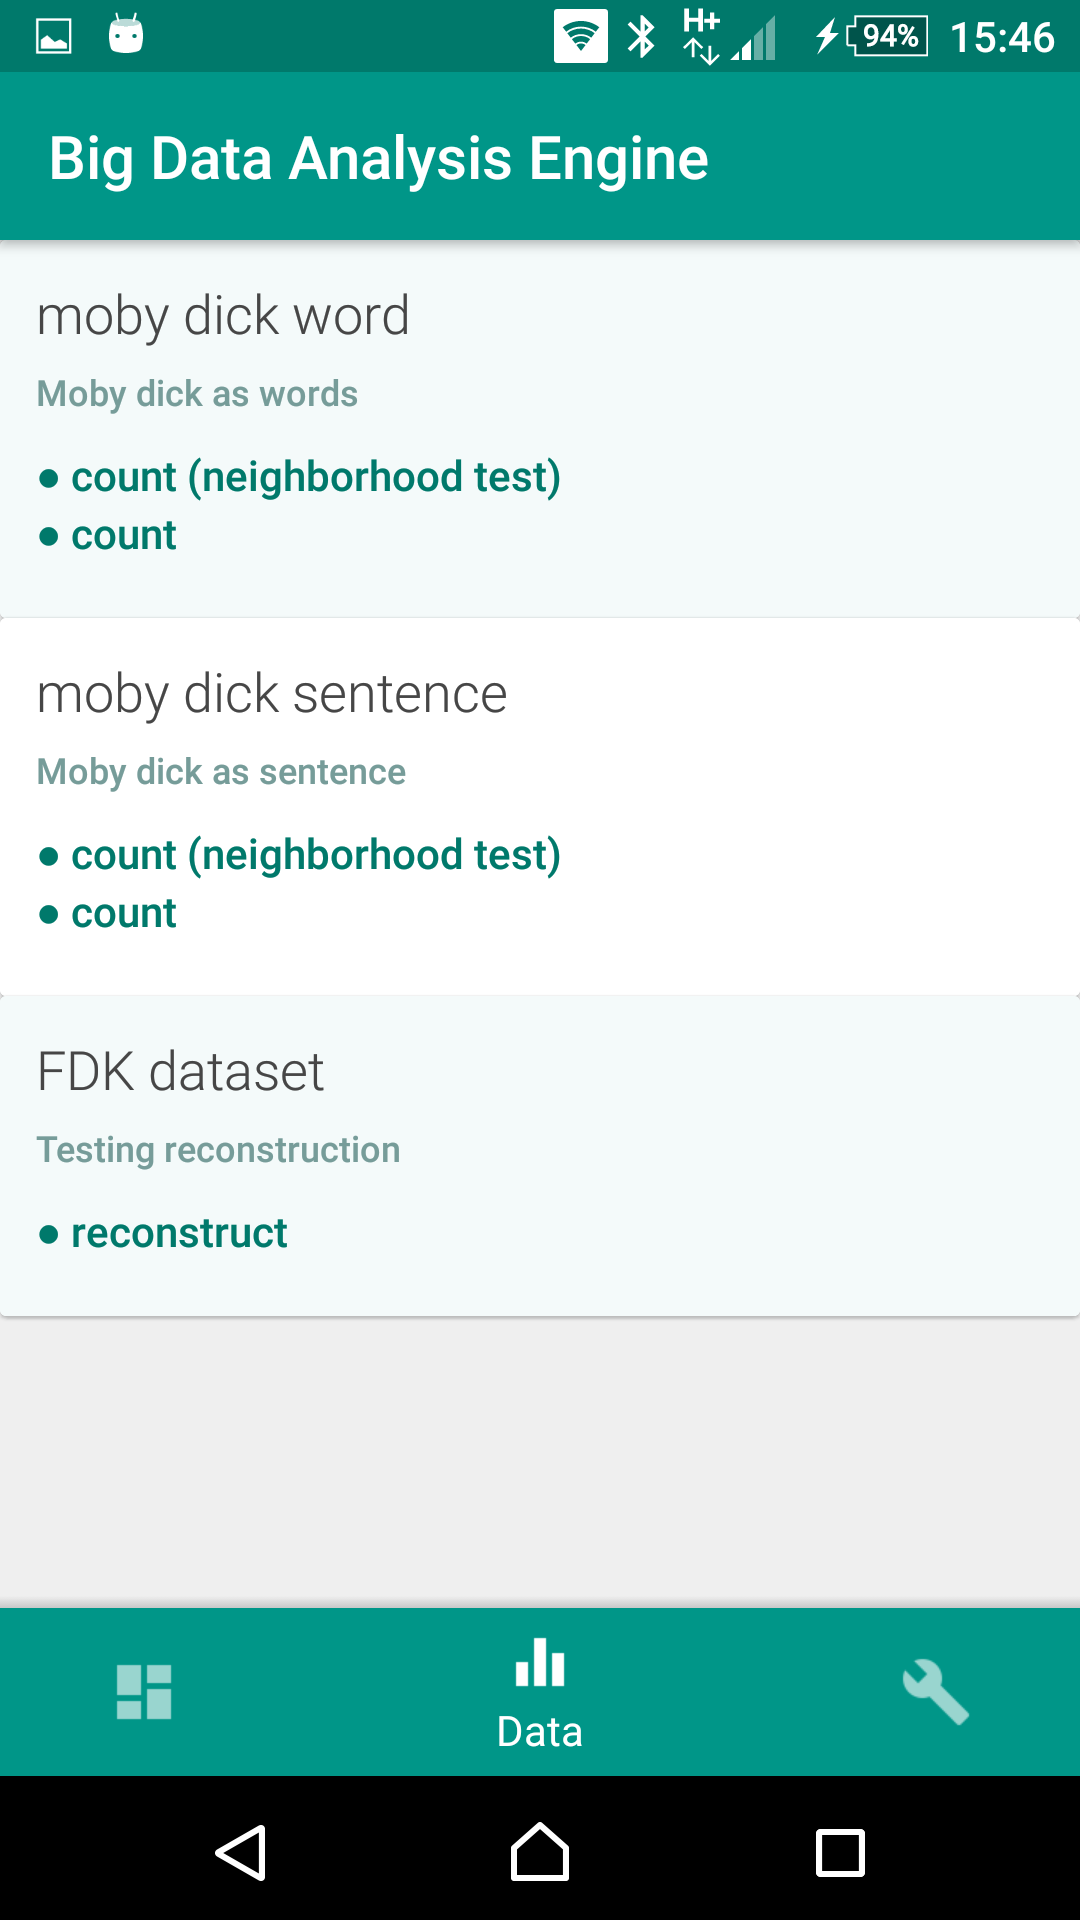
\includegraphics[width=\textwidth]{img/datasets.png}
   	  	\caption[]{List of available datasets and their associated operations.}
    \end{minipage}
  	\hfill
  	\begin{minipage}[b]{0.4\textwidth}
    		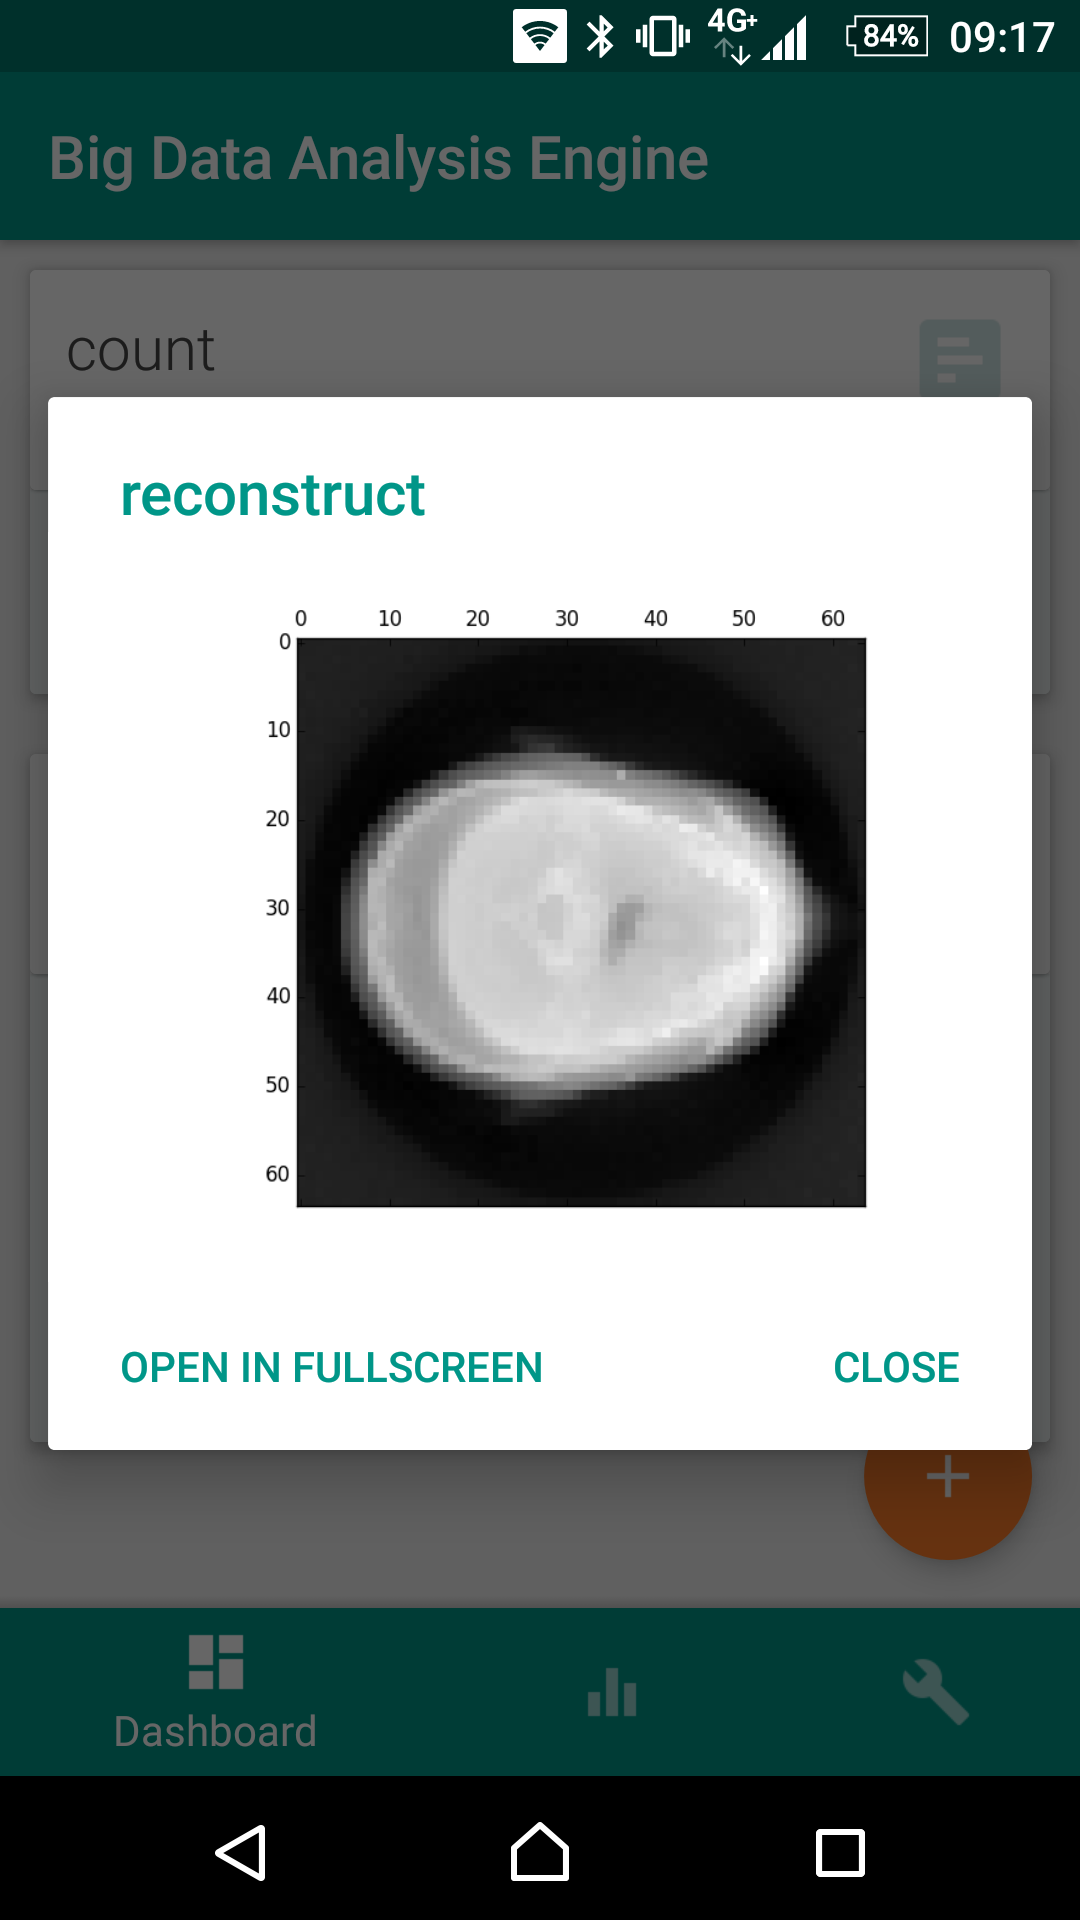
\includegraphics[width=\textwidth]{img/result.png}
    		\caption[]{A dialog displaying the result of a CT reconstruction operation.}
  	\end{minipage}
\end{figure*}

\chapter{Benchmark Graphs}
\section{CT reconstruction} \label{app:fdk}
\begin{figure}[h!]
	\centering
	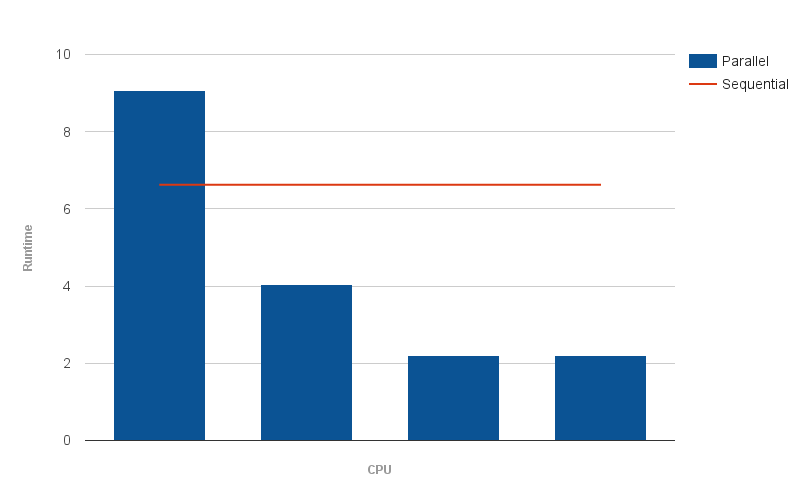
\includegraphics[scale=0.4]{img/fdk-64.png}
	\caption[]{Execution time of the 64x64x64 voxels dataset. \label{fig:fdk-64}}
\end{figure}

\begin{figure}[h!]
	\centering
	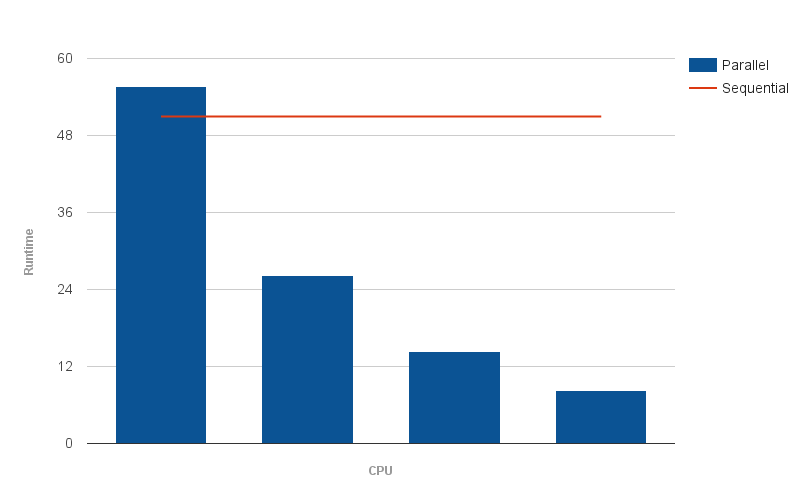
\includegraphics[scale=0.4]{img/fdk-128.png}
	\caption[]{Execution time of the 128x128x128 voxels dataset. \label{fig:fdk-128}}
\end{figure}

\begin{figure}[h!]
	\centering
	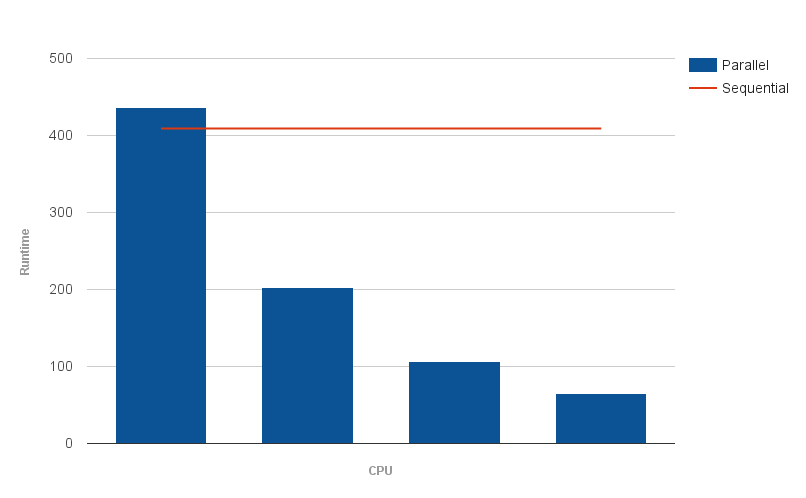
\includegraphics[scale=0.4]{img/fdk-256.png}
	\caption[]{Execution time of the 256x256x256 voxels dataset. \label{fig:fdk-256}}
\end{figure}

\chapter{Hadoop Source Code Example}
\definecolor{pblue}{rgb}{0.13,0.13,1}
\definecolor{pgreen}{rgb}{0,0.5,0}
\definecolor{pred}{rgb}{0.9,0,0}
\definecolor{pgrey}{rgb}{0.46,0.45,0.48}

\section{Map} \label{sec:hadoop-map}
\begin{lstlisting}[language=Java, commentstyle=\color{pgreen}, keywordstyle=\color{pblue}, stringstyle=\color{pred},basicstyle=\fontsize{6}{5}\selectfont\ttfamily, xleftmargin=0.8cm]
package com.cloudera.example;

import org.apache.hadoop.io.IntWritable;
import org.apache.hadoop.io.LongWritable;
import org.apache.hadoop.io.Text;
import org.apache.hadoop.mapreduce.Mapper;

import java.io.IOException;

public class LogEventParseMapper extends Mapper<LongWritable, Text, Text, IntWritable> {
    
    enum Level { TRACE, DEBUG, INFO, WARN, ERROR, FATAL };

    @Override
    public void map(LongWritable key, Text value, Context context)
            throws IOException, InterruptedException {

        String line = value.toString();

        // ignore empty lines
        if (line.trim().isEmpty()) {
            return;
        }
        String[] fields = line.split(" ");

        // ensure this line is not malformed
        if (fields.length <= 3) {
            return;
        }

        String levelField = fields[3];
        for (Level level : Level.values()) {
            String levelName = level.name();
            if (levelName.equalsIgnoreCase(levelField)) {
                context.write(new Text(levelName), new IntWritable(1));
            }
        }
    }
}
\end{lstlisting}
\newpage
\section{Reduce} \label{sec:hadoop-reduce}
\begin{lstlisting}[language=Java, commentstyle=\color{pgreen}, keywordstyle=\color{pblue}, stringstyle=\color{pred},basicstyle=\fontsize{6}{5}\selectfont\ttfamily, xleftmargin=0.8cm]
package com.cloudera.example;

import java.io.IOException;

import org.apache.hadoop.io.IntWritable;
import org.apache.hadoop.io.Text;
import org.apache.hadoop.mapreduce.Reducer;

public class LogEventSumReducer extends Reducer<Text, IntWritable, Text, IntWritable> {

    @Override
    public void reduce(Text key, Iterable<IntWritable> values, Context context) 
            throws IOException, InterruptedException {

        // used to count the number of messages for this event type
        int sum = 0;
        // increment it for each new value received
        for (IntWritable value : values) {
            sum += value.get();
        }

        // Our output is the event type (key) and the sum (value)
        context.write(key, new IntWritable(sum));
    }
}
\end{lstlisting}

\backmatter
\renewcommand*{\printchaptertitle}[1]{\flushleft\chaptitlefont#1}
\renewcommand*{\chaptitlefont}{\normalfont\sffamily\Huge\bfseries}
\chaptermark{Bibliography}
\renewcommand{\sectionmark}[1]{\markright{#1}}
\sectionmark{Bibliography}
\bibliographystyle{ieeetr}
\bibliography{tex/references}

\end{document}